% Options for packages loaded elsewhere
\PassOptionsToPackage{unicode}{hyperref}
\PassOptionsToPackage{hyphens}{url}
\PassOptionsToPackage{dvipsnames,svgnames,x11names}{xcolor}
%
\documentclass[
  letterpaper,
  DIV=11,
  numbers=noendperiod]{scrreprt}

\usepackage{amsmath,amssymb}
\usepackage{iftex}
\ifPDFTeX
  \usepackage[T1]{fontenc}
  \usepackage[utf8]{inputenc}
  \usepackage{textcomp} % provide euro and other symbols
\else % if luatex or xetex
  \usepackage{unicode-math}
  \defaultfontfeatures{Scale=MatchLowercase}
  \defaultfontfeatures[\rmfamily]{Ligatures=TeX,Scale=1}
\fi
\usepackage{lmodern}
\ifPDFTeX\else  
    % xetex/luatex font selection
\fi
% Use upquote if available, for straight quotes in verbatim environments
\IfFileExists{upquote.sty}{\usepackage{upquote}}{}
\IfFileExists{microtype.sty}{% use microtype if available
  \usepackage[]{microtype}
  \UseMicrotypeSet[protrusion]{basicmath} % disable protrusion for tt fonts
}{}
\makeatletter
\@ifundefined{KOMAClassName}{% if non-KOMA class
  \IfFileExists{parskip.sty}{%
    \usepackage{parskip}
  }{% else
    \setlength{\parindent}{0pt}
    \setlength{\parskip}{6pt plus 2pt minus 1pt}}
}{% if KOMA class
  \KOMAoptions{parskip=half}}
\makeatother
\usepackage{xcolor}
\setlength{\emergencystretch}{3em} % prevent overfull lines
\setcounter{secnumdepth}{5}
% Make \paragraph and \subparagraph free-standing
\makeatletter
\ifx\paragraph\undefined\else
  \let\oldparagraph\paragraph
  \renewcommand{\paragraph}{
    \@ifstar
      \xxxParagraphStar
      \xxxParagraphNoStar
  }
  \newcommand{\xxxParagraphStar}[1]{\oldparagraph*{#1}\mbox{}}
  \newcommand{\xxxParagraphNoStar}[1]{\oldparagraph{#1}\mbox{}}
\fi
\ifx\subparagraph\undefined\else
  \let\oldsubparagraph\subparagraph
  \renewcommand{\subparagraph}{
    \@ifstar
      \xxxSubParagraphStar
      \xxxSubParagraphNoStar
  }
  \newcommand{\xxxSubParagraphStar}[1]{\oldsubparagraph*{#1}\mbox{}}
  \newcommand{\xxxSubParagraphNoStar}[1]{\oldsubparagraph{#1}\mbox{}}
\fi
\makeatother

\usepackage{color}
\usepackage{fancyvrb}
\newcommand{\VerbBar}{|}
\newcommand{\VERB}{\Verb[commandchars=\\\{\}]}
\DefineVerbatimEnvironment{Highlighting}{Verbatim}{commandchars=\\\{\}}
% Add ',fontsize=\small' for more characters per line
\usepackage{framed}
\definecolor{shadecolor}{RGB}{241,243,245}
\newenvironment{Shaded}{\begin{snugshade}}{\end{snugshade}}
\newcommand{\AlertTok}[1]{\textcolor[rgb]{0.68,0.00,0.00}{#1}}
\newcommand{\AnnotationTok}[1]{\textcolor[rgb]{0.37,0.37,0.37}{#1}}
\newcommand{\AttributeTok}[1]{\textcolor[rgb]{0.40,0.45,0.13}{#1}}
\newcommand{\BaseNTok}[1]{\textcolor[rgb]{0.68,0.00,0.00}{#1}}
\newcommand{\BuiltInTok}[1]{\textcolor[rgb]{0.00,0.23,0.31}{#1}}
\newcommand{\CharTok}[1]{\textcolor[rgb]{0.13,0.47,0.30}{#1}}
\newcommand{\CommentTok}[1]{\textcolor[rgb]{0.37,0.37,0.37}{#1}}
\newcommand{\CommentVarTok}[1]{\textcolor[rgb]{0.37,0.37,0.37}{\textit{#1}}}
\newcommand{\ConstantTok}[1]{\textcolor[rgb]{0.56,0.35,0.01}{#1}}
\newcommand{\ControlFlowTok}[1]{\textcolor[rgb]{0.00,0.23,0.31}{\textbf{#1}}}
\newcommand{\DataTypeTok}[1]{\textcolor[rgb]{0.68,0.00,0.00}{#1}}
\newcommand{\DecValTok}[1]{\textcolor[rgb]{0.68,0.00,0.00}{#1}}
\newcommand{\DocumentationTok}[1]{\textcolor[rgb]{0.37,0.37,0.37}{\textit{#1}}}
\newcommand{\ErrorTok}[1]{\textcolor[rgb]{0.68,0.00,0.00}{#1}}
\newcommand{\ExtensionTok}[1]{\textcolor[rgb]{0.00,0.23,0.31}{#1}}
\newcommand{\FloatTok}[1]{\textcolor[rgb]{0.68,0.00,0.00}{#1}}
\newcommand{\FunctionTok}[1]{\textcolor[rgb]{0.28,0.35,0.67}{#1}}
\newcommand{\ImportTok}[1]{\textcolor[rgb]{0.00,0.46,0.62}{#1}}
\newcommand{\InformationTok}[1]{\textcolor[rgb]{0.37,0.37,0.37}{#1}}
\newcommand{\KeywordTok}[1]{\textcolor[rgb]{0.00,0.23,0.31}{\textbf{#1}}}
\newcommand{\NormalTok}[1]{\textcolor[rgb]{0.00,0.23,0.31}{#1}}
\newcommand{\OperatorTok}[1]{\textcolor[rgb]{0.37,0.37,0.37}{#1}}
\newcommand{\OtherTok}[1]{\textcolor[rgb]{0.00,0.23,0.31}{#1}}
\newcommand{\PreprocessorTok}[1]{\textcolor[rgb]{0.68,0.00,0.00}{#1}}
\newcommand{\RegionMarkerTok}[1]{\textcolor[rgb]{0.00,0.23,0.31}{#1}}
\newcommand{\SpecialCharTok}[1]{\textcolor[rgb]{0.37,0.37,0.37}{#1}}
\newcommand{\SpecialStringTok}[1]{\textcolor[rgb]{0.13,0.47,0.30}{#1}}
\newcommand{\StringTok}[1]{\textcolor[rgb]{0.13,0.47,0.30}{#1}}
\newcommand{\VariableTok}[1]{\textcolor[rgb]{0.07,0.07,0.07}{#1}}
\newcommand{\VerbatimStringTok}[1]{\textcolor[rgb]{0.13,0.47,0.30}{#1}}
\newcommand{\WarningTok}[1]{\textcolor[rgb]{0.37,0.37,0.37}{\textit{#1}}}

\providecommand{\tightlist}{%
  \setlength{\itemsep}{0pt}\setlength{\parskip}{0pt}}\usepackage{longtable,booktabs,array}
\usepackage{calc} % for calculating minipage widths
% Correct order of tables after \paragraph or \subparagraph
\usepackage{etoolbox}
\makeatletter
\patchcmd\longtable{\par}{\if@noskipsec\mbox{}\fi\par}{}{}
\makeatother
% Allow footnotes in longtable head/foot
\IfFileExists{footnotehyper.sty}{\usepackage{footnotehyper}}{\usepackage{footnote}}
\makesavenoteenv{longtable}
\usepackage{graphicx}
\makeatletter
\def\maxwidth{\ifdim\Gin@nat@width>\linewidth\linewidth\else\Gin@nat@width\fi}
\def\maxheight{\ifdim\Gin@nat@height>\textheight\textheight\else\Gin@nat@height\fi}
\makeatother
% Scale images if necessary, so that they will not overflow the page
% margins by default, and it is still possible to overwrite the defaults
% using explicit options in \includegraphics[width, height, ...]{}
\setkeys{Gin}{width=\maxwidth,height=\maxheight,keepaspectratio}
% Set default figure placement to htbp
\makeatletter
\def\fps@figure{htbp}
\makeatother

\KOMAoption{captions}{tableheading}
\makeatletter
\@ifpackageloaded{tcolorbox}{}{\usepackage[skins,breakable]{tcolorbox}}
\@ifpackageloaded{fontawesome5}{}{\usepackage{fontawesome5}}
\definecolor{quarto-callout-color}{HTML}{909090}
\definecolor{quarto-callout-note-color}{HTML}{0758E5}
\definecolor{quarto-callout-important-color}{HTML}{CC1914}
\definecolor{quarto-callout-warning-color}{HTML}{EB9113}
\definecolor{quarto-callout-tip-color}{HTML}{00A047}
\definecolor{quarto-callout-caution-color}{HTML}{FC5300}
\definecolor{quarto-callout-color-frame}{HTML}{acacac}
\definecolor{quarto-callout-note-color-frame}{HTML}{4582ec}
\definecolor{quarto-callout-important-color-frame}{HTML}{d9534f}
\definecolor{quarto-callout-warning-color-frame}{HTML}{f0ad4e}
\definecolor{quarto-callout-tip-color-frame}{HTML}{02b875}
\definecolor{quarto-callout-caution-color-frame}{HTML}{fd7e14}
\makeatother
\makeatletter
\@ifpackageloaded{bookmark}{}{\usepackage{bookmark}}
\makeatother
\makeatletter
\@ifpackageloaded{caption}{}{\usepackage{caption}}
\AtBeginDocument{%
\ifdefined\contentsname
  \renewcommand*\contentsname{Table of contents}
\else
  \newcommand\contentsname{Table of contents}
\fi
\ifdefined\listfigurename
  \renewcommand*\listfigurename{List of Figures}
\else
  \newcommand\listfigurename{List of Figures}
\fi
\ifdefined\listtablename
  \renewcommand*\listtablename{List of Tables}
\else
  \newcommand\listtablename{List of Tables}
\fi
\ifdefined\figurename
  \renewcommand*\figurename{Figure}
\else
  \newcommand\figurename{Figure}
\fi
\ifdefined\tablename
  \renewcommand*\tablename{Table}
\else
  \newcommand\tablename{Table}
\fi
}
\@ifpackageloaded{float}{}{\usepackage{float}}
\floatstyle{ruled}
\@ifundefined{c@chapter}{\newfloat{codelisting}{h}{lop}}{\newfloat{codelisting}{h}{lop}[chapter]}
\floatname{codelisting}{Listing}
\newcommand*\listoflistings{\listof{codelisting}{List of Listings}}
\makeatother
\makeatletter
\makeatother
\makeatletter
\@ifpackageloaded{caption}{}{\usepackage{caption}}
\@ifpackageloaded{subcaption}{}{\usepackage{subcaption}}
\makeatother

\ifLuaTeX
  \usepackage{selnolig}  % disable illegal ligatures
\fi
\usepackage{bookmark}

\IfFileExists{xurl.sty}{\usepackage{xurl}}{} % add URL line breaks if available
\urlstyle{same} % disable monospaced font for URLs
\hypersetup{
  pdftitle={AI assistants for Scientific Coding},
  pdfauthor={Chris Brown},
  colorlinks=true,
  linkcolor={blue},
  filecolor={Maroon},
  citecolor={Blue},
  urlcolor={Blue},
  pdfcreator={LaTeX via pandoc}}


\title{AI assistants for Scientific Coding}
\author{Chris Brown}
\date{2027-06-08}

\begin{document}
\maketitle

\renewcommand*\contentsname{Table of contents}
{
\hypersetup{linkcolor=}
\setcounter{tocdepth}{2}
\tableofcontents
}

\bookmarksetup{startatroot}

\chapter{Summary}\label{summary}

If you are doing data analysis you are probably using language models
(e.g.~ChatGPT) to help you write code, but are you using them in the
most effective way? Language models have different biases to humans and
so make different types of errors. This book will cover how to use
language models to learn scientific computing and conduct reliable
environmental analyses. The book is reference material for a 1-day
workshop I teach.

I will cover:

\begin{itemize}
\item
  How to use different software tools from the simple interfaces like
  ChatGPT to advanced tools that can run and test code by themselves and
  keep going until the analysis is complete (and even written up).
\item
  Vibe coding and how future analysis workflows will change dramatically
  from today
\item
  Best practice prompting techniques that can dramatically improve model
  performance for complex data analysis
\item
  Applying language models to common environmental applications such as
  GLMs and multivariate statistics
\item
  Issues including environmental impacts, copyright and ethics
\item
  I'll also make space for an interactive discussion of people's
  concerns about AI, but also the opportunities.
\end{itemize}

The content I'll teach is suitable for anyone using computing coding
(e.g.~R, Python) to do data analysis.

Examples will be in marine conservation science using the R language,
but the methods are general to any field. The AI software is also
general to any programming language and we won't be doing much actual
coding (the AI does that!) so participants can follow along in other
languages if they prefer. To follow the practical applications you will
need to have some experience in scientific computing (e.g.~R or Python).

\subsubsection{Who should read this
book?}\label{who-should-read-this-book}

The book is for: anyone who currently uses R, from intermittent users to
experienced professionals. The workshop is not suitable for those that
need an introduction to R and I'll assume students know at least what R
does and are able to do tasks like read in data and create plots.

Important This book isn't for people who need an introduction to R or
Python. I'll assume students know at least how to do tasks like read in
data and create plots in Python or R. To use these AI tools effectively
you absolutely have to understand how scientific computing works first.
If you need an introduction to R then I recommend you learn it without
AI first.

\section{About Chris}\label{about-chris}

I'm an Associate Professor of Fisheries Science at University of
Tasmania and an Australian Research Council Future Fellow. I specialise
in data analysis and modelling, skills I use to better inform
environmental decision makers. R takes me many places and I've worked
with marine ecosystems from tuna fisheries to mangrove forests. I'm an
experienced teacher of R. I have taught R to 100s people over the years,
from the basics to sophisticated modelling and for everyone from
undergraduates to my own supervisors.

\section{Citation for book}\label{citation-for-book}

If following the prompting advice please consider citing my accompanying
article, currently in pre-print form:

\textbf{Citation: Brown \& Spillias (2025). Prompting large language
models for quality ecological statistics. Pre-print.
https://doi.org/10.32942/X2CS80}

\section{Software you'll need for this
workshop}\label{software-youll-need-for-this-workshop}

Save some time for setting up the software, there is a bit to it. You
may also need IT help if your computer is locked down. See the
Chapter~\ref{sec-setup} for more detailed instructions.

\section{Book overview}\label{book-overview}

Note the book isn't currently complete. I've just posted this so
workshop attendees can use the set-up instructions in
Chapter~\ref{sec-setup}.
\href{https://www.seascapemodels.org/R-llm-workshop/index.html}{Here's
an earlier version of the book that is finished.}

\textbf{Part 1} Generative AI for research applications

Chapters 4-5 deal with the basics of prompting LLMs, as well as some
more advanced research applications such as systematic literature
reviewers and automating topic research.

\textbf{Part 2} Generative AI coding assistants for scientific
computation

In chapters 6-8 we'll look at how you can use coding assistants to
improve your scientific coding. These chapters will make use of Github
Copilot, those other AI coding assistants can also be used.

\textbf{Part 3}

We'll discuss ethics, copyright, costs and security in chapters 9-10.

\section{Data}\label{data}

We'll load all data files directly via URL in the workshop notes. So no
need to download any data now. Details on data attribution are below.

\subsection{Benthic cover surveys and fish
habitat}\label{benthic-cover-surveys-and-fish-habitat}

In this course we'll be analyzing benthic cover and fish survey data.
These data were collected by divers doing standardized surveys on the
reefs of Kia, Solomon Islands. These data were first publshed by
\href{http://dx.doi.org/10.1016/j.biocon.2017.04.024}{Hamilton et
al.~2017} who showed that logging of forests is causing sedimentation
and impact habitats of an important fishery species.

In a follow-up study \href{http://dx.doi.org/10.1111/cobi.13079}{Brown
and Hamilton 2018} developed a Bayesian model that estimates the size of
the footprint of pollution from logging on reefs.

\bookmarksetup{startatroot}

\chapter{Introduction to LLMs for R}\label{introduction-to-llms-for-r}

\textbf{Time:} 9-10am

In this presentation I'll cover how LLMs work, best practices prompt
engineering, software, applications for R users and ethics.

This chapter provides an overview of:

\begin{itemize}
\tightlist
\item
  How Large Language Models (LLMs) function and their capabilities
\item
  Best practices for prompt engineering when working with R
\item
  Software options available for R users to interact with LLMs (coding
  assistants)
\item
  Practical applications of LLMs for R programming and data analysis
\item
  Ethical considerations when using LLMs for scientific work
\end{itemize}

We'll explore how LLMs can enhance your R workflow, from code generation
to data analysis assistance, while maintaining scientific rigor and
reproducibility.

\href{https://docs.google.com/presentation/d/1BYfAjU4NPaIQ9CNSRlIVZJpJGof3moS9/edit?usp=drive_link&ouid=107596646496267980935&rtpof=true&sd=true}{Slides
for presentation (on a google drive)}

\section{The jagged frontier of LLM
progress}\label{the-jagged-frontier-of-llm-progress}

LLMs were created to write text. But it soon became apparent that they
excel at writing programming code in many different languages.

Since then AI companies have been optimising their training and
development for coding and logic.

There are a series of standardized tests that are used to compare
quality of LLMs. Common evaluation tests are the SWE benchmark which
looks at the ability of LLMs to autonomously create bug fixes. Current
models get about \href{https://www.swebench.com/}{50\% resolution on
this benchmark}.

Their progress on math and logic is a bit more controversial. It seems
like some of the math benchmarks (like AIME annual tests for top 5\%
highschool students)
\href{https://epoch.ai/frontiermath/the-benchmark}{are saturated as LLMs
are scoring close to 100\% on these tests.}. So newer tests of unsolved
maths problems are being developed.

However, others are finding that the ability of
\href{https://garymarcus.substack.com/p/reports-of-llms-mastering-math-have}{LLMs
on math and logic are overstated}, perhaps because the LLMs have been
trained on the questions and the answers. Its also clear that AI
companies have a strong financial incentive to find ways (real and
otherwise) of improving on the benchmarks. Are the moment there is tough
competition to be `industry leaders' and grab market share with
impressive results on benchmarks.

Either way, it does seem that the current areas of progress are
programming, math and logic.

Evaluations on statistics and the R software are less common.

The limited evaluations of LLMs on their ability to identify the correct
statistical procedure are less impressive than other benchmarks.
\href{https://arxiv.org/abs/2406.07815}{An evaluation (published 2025)
of several models, including GPT-4 as the most up-to-date model}, found
accuracy at suggesting the correct statistical test of between 8\% and
90\%.

In general LLMs were good at choosing descriptive statistics (accuracy
of up to 90\% for GPT-4). Whereas when choosing inferential tests
accuracy was much less impressive - GPT-4 scored between 20\% and 43\%
accuracy on questions for which a contingency table was the correct
answer.

The results also indicate the improvements that can be gained through
better prompts (i.e.~doubling in accuracy for GPT 4).

The lesson is two-fold. Just because LLMs excel at some tasks doesn't
mean they will excel at others. Second, good prompting strategies pay
off.

For us in the niche R world there is also another lesson. The LLMs
should be good at helping us implement analyses (ie write the R code).
However, they are less reliable as statisticians who can guide us on the
scientific question of what type of analysis to do.

\bookmarksetup{startatroot}

\chapter{Software you'll need for this book and how to set it
up}\label{sec-setup}

There's lots of options for AI coding assistant software. What you use
will depend on:

\begin{itemize}
\tightlist
\item
  Whether you are using R or Python
\item
  Your level of coding experience
\item
  Your IT capabilities for setting up software
\item
  What you budget for AI is
\end{itemize}

Below I've provided instructions for some of the options. These
certainly aren't comprehensive.

I recommend following this page from a computer, not a mobile device.
The right hand menu will show and has the navigation pane so you can
jump to the section that's relevant to your set-up needs.

\section{R packages}\label{r-packages}

If you are using R then we will make use of:
\texttt{install.packages(c("vegan",\ "ellmer","tidyverse")}. For Python
users you can follow along most examples without these, this isn't an R
training course, its an course on using AI to assist with coding.

\section{Options for AI software}\label{options-for-ai-software}

\subsection{Preferred option for R
users}\label{preferred-option-for-r-users}

What I will be using, and what I prefer you to use is:

\begin{itemize}
\tightlist
\item
  The R program from the VS Code Integrated Development Environment
  (IDE)
\item
  Github Copilot
\item
  R Ellmer package, for which you'll need an API key to one of the LLM
  providers
\end{itemize}

The challenges with the above options are that it can sometimes be
difficult to connect R and VScode. Comprehensive instructions are below.
You may need IT help, especially if your computer is locked down!

If you chose this option you will need to follow instructions in this
chapter for `Getting an API key' (Section~\ref{sec-apikeys}) (required
for ellmer), `Ellmer set-up' (Section~\ref{sec-ellmer}), VS code setup
(Section~\ref{sec-vscodesetup}) and `Github Copilot set-up'
(Section~\ref{sec-githubcopilot}).

\subsection{Option 2 for R users}\label{option-2-for-r-users}

Use Rstudio with R. You will need \texttt{ellmer} and \texttt{gander}
packages. See instructions below for `Getting an API key'
(Section~\ref{sec-apikeys}), `Ellmer set-up' (Section~\ref{sec-ellmer})
and `Gander: Rstudio friendly alternative to copilot'
(Section~\ref{sec-gander}).

Rstudio also has basic Github Copilot capablities. To use these (not
essential for the workshop) get a copilot account
(Section~\ref{sec-githubcopilot}) then in Rstudio go to `Tools'
-\textgreater{} `Global Options' -\textgreater{} `Copilot' and enable it
(follow instructions for entering password to setup).

\subsection{Python users}\label{python-users}

I'm not a Python programmer, however, all the principles I'll teach also
apply to Python. You can easily follow on with the examples in Python.

You will need to have VSCode with Github Copilot. So I recommend you get
the VScode software, then follow these instructions for
\href{https://code.visualstudio.com/docs/python/python-tutorial}{Python
set-up}.

Then follow the instructions for `Github Copilot set-up'
(Section~\ref{sec-githubcopilot}).

I also recommend you get an API key with OpenRouter
(Section~\ref{sec-apikeys}).

You don't need an ellmer equivalent because most of the LLM providers
already provide Python code on their webpages.

\subsection{Options 3 +}\label{options-3}

There are innumerable AI coding assistants now available. Feel free to
BYO if you are using one that you are already comfortable with. However,
I strongly recommend using a tool with IDE integration (meaning it can
edit your R/Python scripts directly). See
Section~\ref{sec-otheroptions}.

As a fall-back, you can follow this course via ChatGPT or Copilot, but
it will lots of cutting and pasting. Not the integrated experience I
want you to have.

\section{Software options summary}\label{software-options-summary}

Here are some of the software options I've looked at. Or if you've
picked your option from the above list, just jump ahead to the required
sections.

\begin{longtable}[]{@{}
  >{\raggedright\arraybackslash}p{(\columnwidth - 6\tabcolsep) * \real{0.0456}}
  >{\raggedright\arraybackslash}p{(\columnwidth - 6\tabcolsep) * \real{0.1298}}
  >{\raggedright\arraybackslash}p{(\columnwidth - 6\tabcolsep) * \real{0.6316}}
  >{\raggedright\arraybackslash}p{(\columnwidth - 6\tabcolsep) * \real{0.1930}}@{}}
\toprule\noalign{}
\begin{minipage}[b]{\linewidth}\raggedright
Option
\end{minipage} & \begin{minipage}[b]{\linewidth}\raggedright
Best for
\end{minipage} & \begin{minipage}[b]{\linewidth}\raggedright
Pros
\end{minipage} & \begin{minipage}[b]{\linewidth}\raggedright
Cons
\end{minipage} \\
\midrule\noalign{}
\endhead
\bottomrule\noalign{}
\endlastfoot
VScode with Github Copilot & Coders of all abilities who have a fixed
budget or just want to try IDE integration & - Subscription based-
Capable free tier- Editor integration (auto-complete style)- Agent mode-
Multiple LLMs available- Easy to use & - VSCode can be hard to set-up
for R users- Less flexibility and customization than other agents- The
Github Copilot Agent is less automated than other agent software-
Limited choice of LLMs (unless you BYO API key) \\
Ellmer R package & R users who want to create their own chat bots, or
integrate LLMs into their code and shiny apps. For example, to extract
data from a large corpus of papers. & - Works anywhere R works-
Unlimited flexibility- BYO API key, can interact with any LLM- Automate
API calls to LLMs & - Only a basic prompt interface provided (you need
to write it) \\
Gander R package & Moderately experienced R users who don't want to
leave RStudio. & - Works with Rstudio- Can see `inside of' R objects, so
knows your variable names- Can customize how it works to optimize
performance and cost- BYO API key, can interact with any LLM & -
Requires some experience with the R program- Not as deeply integrated
with Rstudio as Github Copilot is with VScode (doesn't have as many
features as copilot) \\
Aider & Experienced python programmers & - Python based AI agent-
Interact with the agent via Python code- Highly flexible, can use as an
everyday coding assistant or to create bespoke agents- Can edit files as
well as run in agent mode & - Not a straightforward prompt interface-
Requires Python coding experience \\
VSCode with Roo Code & Experienced programmers who want to fully
automate coding workflows & - Fully automated agents- Multiple modes for
different behaviours, e.g.~architect versus code- Orchestrate mode that
can delegate to sub-agents and complete very complex tasks- BYO API key-
System messages fully customizable for advanced scientific applications
of agents- One of the best performing and most popular agents & - VSCode
can be hard to set-up for R users- Can get more expensive- Does not do
inline code editing `as you type' like copilot- Not suitable for novice
programmers \\
VSCode with Cline & Same as Roo Code. The user base for Cline is
slightly larger. & - Fully automated agents- Multiple modes for
different behaviours- BYO API key- System messages customizable- Large
user base & - Less options for customizing the system prompt compared to
Roo Code- Not suitable for novice programmers \\
Positron with Roo Code or Cline & R users who don't want to use VScode.
Positron is a fork (copy) of VScode managed by Posit, the group who run
RStudio. & - Possibly a bit easier to set-up R than with VScode- Pros
and cons are same as VScode with Roo Code or Cline & - New software-
Limited features and support \\
\end{longtable}

There are many other (10s, 100s?) of coding assistants now available.
Some prominent examples are Claude code, Cursor and Windsurf. I haven't
tried these, I understand they are similar to Github Copilot. Last time
I checked none of them worked with Rstudio.

\section{Getting an API key}\label{sec-apikeys}

An API key is like a password that allows the AI assistant (e.g.~roo
code) to send your prompt to a large language model. Your key should be
kept private. Usually you'll have to buy some credits. These allow you
to send prompts to the LLM. You'll be paying per prompt.

Now you need to choose your large language model provider. I'm currently
using OpenRouter and Anthropic, which have a diversity of models for
generating text, code and reading images. Do some web searching to find
out the latest info on providers and models.

You choose depends on what you want to do and your budget. Some
providers offer a free tier. You'll need to web search for the latest
info on this.

For this workshop I \textbf{strongly recommend you get an OpenRouter API
key}. This will give you the most flexibility to try different models
and to find models that have free options.

Once you've chosen a provider, create an account and follow their
instructions for creating an API key. You will probably also need to buy
some credit to use the model.

The one caveat is that OpenRouter may not have access the the full
capabilities of all LLMs. For example, when Sonnet 3.7 came out you
could get vision capabilities via an Anthropic API key but not with an
OpenRouter API key.

\textbf{Important} the sign-up for getting an API key is often through a
different webpage to the sign-up you may be using for subscription based
AI tools (e.g.~Claude Code or ChatGPT). Here are a couple of key links:

\begin{itemize}
\tightlist
\item
  \href{https://accounts.openrouter.ai/sign-up}{Sign-up here to get an
  API key for OpenRouter to access LLMs from 100s of providers}
\item
  \href{https://console.anthropic.com/login}{Sign-up here to get an API
  key for Anthropic's LLMs}
\item
  \href{https://auth.openai.com/log-in}{Sign-up here to get an API key
  for OpenAI's LLMs}
\end{itemize}

\section{VSCode set-up for R users}\label{sec-vscodesetup}

VScode has many extensions that let you create and run entire workflows
via using prompts to a large language model. Its not widely used in the
R community yet, but I expect it will be soon. You can create your
entire R project, interpret the results and write a draft of your
findings without writing any R code.

Most of these tools are not available (as of writing) in RStudio, or
have only limited functionality. So you need to use a different IDE
(Integrated Development Environment) to run your R code. Here I'll
explain how to set-up VSCode (a popular IDE) so you can use Cline.

\subsection{Software requirements}\label{software-requirements}

To set up VScode for R and Cline, you'll need:

\begin{itemize}
\tightlist
\item
  R programming language
\item
  VScode text editor
\item
  R extension for VScode
\item
  Cline AI assistant extension for VScode
\end{itemize}

Note that if you computer is controlled centrally by an IT department,
you may need to request admin access to install software, or email IT
and ask for them to come and help you.

\subsection{Install R}\label{install-r}

\begin{enumerate}
\def\labelenumi{\arabic{enumi}.}
\tightlist
\item
  Go to the official R project website: https://www.r-project.org/
\item
  Click the ``download R'' link in the Getting Started section
\item
  Choose a CRAN mirror close to your location
\item
  Download the appropriate R installer for your operating system
\item
  Run the installer and follow the prompts to complete installation
\end{enumerate}

\subsection{R packages}\label{r-packages-1}

\begin{enumerate}
\def\labelenumi{\arabic{enumi}.}
\tightlist
\item
  Open R or RStudio
\item
  Install language server \texttt{install.packages("languageserver")}
\item
  Install httpgd \texttt{install.packages("httpgd")} (this helps improve
  plots in VScode). NOTE that httpgd seems to often be removed from
  CRAN, then come back again, I'm not sure why\ldots{} If you are having
  trouble you can try install from a different repo, see instructions
  here: https://community.r-multiverse.org/httpgd
\end{enumerate}

\subsection{Install VScode}\label{install-vscode}

\begin{enumerate}
\def\labelenumi{\arabic{enumi}.}
\tightlist
\item
  Go to the official VScode website: https://code.visualstudio.com/
\item
  Click the big blue ``Download'' button
\item
  Download the appropriate VScode installer for your operating system
\item
  Run the installer and follow the prompts
\item
  Launch VScode once installation is complete
\end{enumerate}

\subsection{Install R extension}\label{install-r-extension}

\begin{enumerate}
\def\labelenumi{\arabic{enumi}.}
\tightlist
\item
  Open VScode
\item
  Open the Extensions view in VScode (click the boxes on left hand side)
\item
  Search for ``R'' in the extensions marketplace
\item
  Select the ``R'' extension published by REditorSupport
\item
  Click the ``Install'' button
\item
  Restart VScode after installation if prompted
\end{enumerate}

\href{https://code.visualstudio.com/docs/languages/r}{More info on
vscode and R here}

\subsection{Connect R and VScode}\label{connect-r-and-vscode}

\begin{enumerate}
\def\labelenumi{\arabic{enumi}.}
\tightlist
\item
  Open a new terminal in VScode (Terminal \textgreater{} New Terminal)
\item
  Check that R is installed by running: \texttt{R\ -\/-version}
\item
  Type \texttt{R} to open the R console in the terminal
\item
  Now open any R script in VS code (File \textgreater{} Open)
\item
  Run some R code to check that VS code can connect to R in the
  terminal. Use the shortcut Ctrl+Enter/Cmd+Enter or press the play
  button in the top right of the script editor.
\end{enumerate}

If R is not found then open extensions (left hand side, boxes icon),
filter by `enabled' then click the R extension. Now click the cog icon
in the R extension and select `settings' from the dropdown. Search for
`rpath'. Check that it has the correct path to R on your computer. Also
update `rterm' with the same path. You can find the path by opening a
terminal and typing \texttt{which\ R} (on mac) or in a windows terminal
\texttt{where\ R}.

One way to fine out where R is installed on your computer is to open
Rstudio, go to `Tools' -\textgreater{} `General' then under the field `R
version' it will have the path to your R version that may look like
this: `C:\Users\myname\AppData\Progams\R\R-4.5.0'

Copy that path from Rstudio. Then go back to the VScode settings and
paste it into the `rpath' and `rterm' settings. You will also need to
add the \texttt{R.exe} on the end like this:
`C:/Users/myname/AppData/Progams/R/R-4.5.0/R.exe'

Now open an R script and run it (e.g.~press cmd/cntrl-enter). If
everything is connected R will open and it will run the script. If its
not working you'll get an error pop-up. Go back and check the steps
above.

If you copied it on windows you may also need to reverse the slashes,
like I have above.

While you have the extension settings open search for `httgp' and make
sure \texttt{Plot:\ Use\ Httpgd} is enabled.

\subsection{Issues and tips for VScode with
R}\label{issues-and-tips-for-vscode-with-r}

This is just a list of issues I've had and how I've solved them.

\emph{Plotting} If your R plots look weird (like tiny font), make sure
httpgp is enabled. Go back to steps above and see how to do that.

\emph{Viewing data} There are various extensions for viewing csv and
excel files. It is worth looking into these so that when you do
\texttt{View(dat)} in R you get a nice table. Some also allow editing.

\emph{Getting help to install software} My computer is somewhat locked
down by IT, so getting this set-up was a bit fiddly and required a few
requests to IT to install software.

\emph{R markdown} There are options in the R extension settings for how
to knit markdown. You may need to configure these if you want to knit
markdown docs from VScode. If you are having trouble knitting markdown
it may mean that the path to pandoc is not set correctly.
\href{https://stackoverflow.com/questions/60766646/need-help-assigning-global-settings-for-rstudios-pandoc-in-vscode-to-knit-pdf-d}{There
is some helpful instructions here}

\emph{R terminal crashes} If I run too much R code at once (like
selecting a big block then running) the terminal tends to crash.
Initially I see a little highlighted box saying `PTY HOST'. Then I need
to close all the terminals (with the bin icon) and start again. Try
radian if this is a problem. You can also code run line-by-line or
source whole scripts from the terminal (which works fine). I tried
debugging this by increasing the buffer but to on avail.

\emph{Shortcut keys} (on osx) cmd-/ to comment uncomment lines.
cmd-shift-p to open the command palette, cmd-b to open the file
explorer, cmd-enter to run lines or selection of R code, cmd-shift-c to
open terminal in new window, cntrl-shift-` to open a new terminal in vs
code.

\subsection{Installing radian
(optional)}\label{installing-radian-optional}

Radian is a terminal editor that is a bit nicer than the base R one. It
does autocomplete in the terminal (like Rstudio does in the console),
colours code/brackets etc\ldots{} and allows multi-line editing in the
terminal.

To set this up, install radian (you need python to do this). More
\href{https://github.com/randy3k/radian?tab=readme-ov-file}{instructions
here}.

Then go to the terminal and find the path where radian is installed
(e.g.~\texttt{which\ radian} on mac or \texttt{where\ radian} on
windows).

Now open your settings in VScode (cmd-,) and search for `rterm' (stands
for `R Terminal', don't change the rpath which we set just before). Add
the path to radian to the rterm setting. Also search for the setting `R:
Bracketed Paste' and make sure it is enabled.

\section{Github Copilot set-up}\label{sec-githubcopilot}

Once you have VSCode just
\href{https://docs.github.com/en/copilot/how-tos/manage-your-account/get-started-with-a-copilot-plan\#visual-studio-and-vs-code}{follow
the simple steps here}. Note if you already have a Github account make
sure you have your login information handy.

\section{Ellmer set-up}\label{sec-ellmer}

First, you need to get an API key from the provider, see step above on
`Getting an API key'.

Then, you need to add the key to your .Renviron file:

\texttt{usethis::edit\_r\_environ()}

Then type in your key like this:

OPENROUTER\_API\_KEY=``xxxxxx''

If you are using open AI it would be like this:

OPENAI\_API\_KEY=``xxxxxx''

i.e.~use the appropriate name for the provider you are using.

Then restart R. ellmer will automatically find your key so long as you
use the recommended environment variable names. See
?ellmer::chat\_openrouter (or chat\_xxx where xxx is whatever provider
you are using).

\section{Gander: Rstudio friendly alternative to
copilot}\label{sec-gander}

\href{https://simonpcouch.github.io/gander/articles/gander.html}{Gander
lets you select code in Rstudio and edit it directly through calls to an
LLM}.

Follow the steps to set-up Ellmer first.

Then you can \texttt{install.packages(gander)}

Now, you need to do two steps before Gander will work. First you need to
add your default LLM to the .Rprofile so Gander knows what LLM to use
type: \texttt{usethis::edit\_r\_profile()}

Now set the option for your LLM, e.g.~

\texttt{options(.gander\_chat\ =\ ellmer::chat\_anthropic())} or
\texttt{options(.gander\_chat\ =\ ellmer::chat\_openai())}

Now add a keyboard short-cut to use Gander. Go to the `Tools' menu at
the top, click `Add-ins', `Browse Add-ins', then click the `Keyboard
shortcuts' button. Find the row for Gander (probably at the bottom),
click in the second column for `Shortcut' and type your keyboard
shortcut. I used cmd-i (or cntrl-i). Then click `Cancel' once you've set
the shortcut key (`Cancel' as we don't want to run Gander right now).

If for some reason the shortcut key won't you can also
\texttt{gander::gander\_addin()} at anytime from R.

Now to check it works, open an R project and select a line of R code.
Press your shortcut keys. A box should pop up. Type a prompt (like `make
this code more fun') and hit enter to test it does something.

I recommend reading the gander reference as there are ways you can
\href{https://simonpcouch.github.io/gander/articles/gander.html}{customize
it to know your data but also save on tokens}.

\section{Installing other gen AI VSCode
extensions}\label{sec-otheroptions}

e.g.~if you want to try Roo Code or Cline.

\begin{enumerate}
\def\labelenumi{\arabic{enumi}.}
\tightlist
\item
  Open the Extensions view in VScode (Ctrl+Shift+X)
\item
  Search for the genAI assistant of your choice. I'm use Roo Code
  currently. Cline is another popular choice.
\item
  Select the extension
\item
  Click the ``Install'' button
\item
  The extension icon (e.g.~a Roo if using Roo Code) should appear in the
  VScode sidebar (left side).
\end{enumerate}

You'll have to navigate the extensions menus to input your API key. It
won't work without an API key that gives you access to an LLM. e.g.~for
Roo Code:

\begin{enumerate}
\def\labelenumi{\arabic{enumi}.}
\tightlist
\item
  Click on the extension icon (e.g.~a roo for roo code or robot for
  cline) on the left hand side
\item
  Click the cog (if the settings don't open automatically)
\item
  Select your API provider and cut and paste the API key into the box.
\end{enumerate}

\bookmarksetup{startatroot}

\chapter{LLM prompting fundamentals}\label{llm-prompting-fundamentals}

\emph{Start of practical material}

We'll cover LLM prompting theory through practical examples. This
section will give you a deep understanding of how chatbots work and
teach you some advanced prompting skills. By understanding these
technical foundations, you'll be better equipped to leverage LLMs
effectively for your R programming and data analysis tasks, and to
troubleshoot when you're not getting the results you expect.

\textbf{Software requirements:} VScode with R or Rstudio. API key,
ideally to openrouter. R (best with ellmer) or Python.

\section{Setup authorisation}\label{setup-authorisation}

Get your API key, see Section~\ref{sec-apikeys} and then
Section~\ref{sec-ellmer} for connecting that to Ellmer.

If you are using Python, save your API key in a .env file in your
project directory, like this: `OPENROUTER\_API\_KEY=my-key-here

\section{Understanding how LLMs work}\label{understanding-how-llms-work}

Large Language Models (LLMs) operate by predicting the next token in a
sequence, one token at a time. To understand how this works in practice,
we'll call an API directly through computer code.

By accessing the API in this way we get as close to the raw LLM as we
are able. Later on we will use `coding assistants' (e.g.~copilot) which
put another layer of software between you and the LLM.

Try to get it to complete a sentence:

\subsection{R - Ellmer}

\begin{Shaded}
\begin{Highlighting}[]
\FunctionTok{library}\NormalTok{(ellmer)}

\CommentTok{\# Initialize a chat with Claude}
\NormalTok{chat }\OtherTok{\textless{}{-}} \FunctionTok{chat\_openrouter}\NormalTok{(}
  \AttributeTok{system\_prompt =} \StringTok{"You are a helpful assistant."}\NormalTok{,}
  \AttributeTok{model =} \StringTok{"anthropic/claude{-}3.5{-}haiku"}\NormalTok{,}
  \AttributeTok{api\_args =} \FunctionTok{list}\NormalTok{(}\AttributeTok{max\_tokens =} \DecValTok{50}\NormalTok{)}
\NormalTok{)}
\NormalTok{chat}\SpecialCharTok{$}\FunctionTok{chat}\NormalTok{(}\StringTok{"Ecologists like to eat "}\NormalTok{)}
\end{Highlighting}
\end{Shaded}

\subsection{R}

\begin{Shaded}
\begin{Highlighting}[]
\FunctionTok{library}\NormalTok{(jsonlite)}
\FunctionTok{library}\NormalTok{(httr)}
\NormalTok{openrouter\_api\_key }\OtherTok{\textless{}{-}} \FunctionTok{Sys.getenv}\NormalTok{(}\StringTok{"OPENROUTER\_API\_KEY"}\NormalTok{)}
\NormalTok{response }\OtherTok{\textless{}{-}} \FunctionTok{POST}\NormalTok{(}
    \AttributeTok{url =} \StringTok{"https://openrouter.ai/api/v1/chat/completions"}\NormalTok{,}
    \FunctionTok{add\_headers}\NormalTok{(}
      \StringTok{"Content{-}Type"} \OtherTok{=} \StringTok{"application/json"}\NormalTok{,}
      \StringTok{"Authorization"} \OtherTok{=} \FunctionTok{paste}\NormalTok{(}\StringTok{"Bearer"}\NormalTok{, openrouter\_api\_key)}
\NormalTok{    ),}
    \AttributeTok{body =} \FunctionTok{toJSON}\NormalTok{(}\FunctionTok{list}\NormalTok{(}
      \AttributeTok{model =} \StringTok{"anthropic/claude{-}3.5{-}haiku"}\NormalTok{,}
      \AttributeTok{messages =} \FunctionTok{list}\NormalTok{(}
        \FunctionTok{list}\NormalTok{(}
          \AttributeTok{role =} \StringTok{"system"}\NormalTok{,}
          \AttributeTok{content =} \StringTok{"You are a helpful assistant."}
\NormalTok{        ),  }
        \FunctionTok{list}\NormalTok{(}
          \AttributeTok{role =} \StringTok{"user"}\NormalTok{,}
          \AttributeTok{content =} \StringTok{"Ecologists like to eat "}
\NormalTok{        )}
\NormalTok{      )}
\NormalTok{    ), }\AttributeTok{auto\_unbox =} \ConstantTok{TRUE}\NormalTok{),}
    \AttributeTok{encode =} \StringTok{"raw"}
\NormalTok{  )}
\NormalTok{r3 }\OtherTok{\textless{}{-}} \FunctionTok{fromJSON}\NormalTok{(}\FunctionTok{content}\NormalTok{(response, }\StringTok{"text"}\NormalTok{))}
\NormalTok{r3}\SpecialCharTok{$}\NormalTok{choices}\SpecialCharTok{$}\NormalTok{message}\SpecialCharTok{$}\NormalTok{content}
\end{Highlighting}
\end{Shaded}

\subsection{Python}

\begin{Shaded}
\begin{Highlighting}[]
\ImportTok{import}\NormalTok{ requests}
\ImportTok{import}\NormalTok{ json}
\ImportTok{import}\NormalTok{ os}
\ImportTok{from}\NormalTok{ dotenv }\ImportTok{import}\NormalTok{ load\_dotenv}
\NormalTok{load\_dotenv()}

\NormalTok{api\_key }\OperatorTok{=}\NormalTok{ os.getenv(}\StringTok{"OPENROUTER\_API\_KEY"}\NormalTok{)}
\NormalTok{model }\OperatorTok{=} \StringTok{"anthropic/claude{-}3.5{-}haiku"}
\NormalTok{message }\OperatorTok{=} \StringTok{"Ecologists like to eat "}

\NormalTok{response }\OperatorTok{=}\NormalTok{ requests.post(}
\NormalTok{  url}\OperatorTok{=}\StringTok{"https://openrouter.ai/api/v1/chat/completions"}\NormalTok{,}
\NormalTok{  headers}\OperatorTok{=}\NormalTok{\{}
    \StringTok{"Authorization"}\NormalTok{: }\SpecialStringTok{f"Bearer }\SpecialCharTok{\{}\NormalTok{api\_key}\SpecialCharTok{\}}\SpecialStringTok{"}\NormalTok{,}
    \StringTok{"Content{-}Type"}\NormalTok{: }\StringTok{"application/json"}
\NormalTok{  \},}
\NormalTok{  data}\OperatorTok{=}\NormalTok{json.dumps(\{}
    \StringTok{"model"}\NormalTok{: model,}
    \StringTok{"messages"}\NormalTok{: [}
\NormalTok{      \{}
        \StringTok{"role"}\NormalTok{: }\StringTok{"system"}\NormalTok{,}
        \StringTok{"content"}\NormalTok{: }\StringTok{"You are a helpful assistant."}\NormalTok{,}
\NormalTok{      \},}
\NormalTok{      \{}
        \StringTok{"role"}\NormalTok{: }\StringTok{"user"}\NormalTok{,}
        \StringTok{"content"}\NormalTok{: message,}
\NormalTok{      \}}
\NormalTok{    ]}
\NormalTok{  \})}
\NormalTok{)}
\NormalTok{data }\OperatorTok{=}\NormalTok{ response.json()}
\NormalTok{content }\OperatorTok{=}\NormalTok{ data[}\StringTok{\textquotesingle{}choices\textquotesingle{}}\NormalTok{][}\DecValTok{0}\NormalTok{][}\StringTok{\textquotesingle{}message\textquotesingle{}}\NormalTok{][}\StringTok{\textquotesingle{}content\textquotesingle{}}\NormalTok{]}
\NormalTok{content}
\end{Highlighting}
\end{Shaded}

Notice that the model doesn't do what we intend, which is complete the
sentence. LLMs have a built in command to be an assistant. Let's use the
`system prompt' to provide it with strong directions.

\textbf{Tip:} The system prompt sets the overall context for a chat. It
is meant to be a stronger directive than the user prompt. In most chat
interfaces (e.g.~copilot) you are interacting with the user prompt. The
provider has provided the system prompt,
\href{https://www.reddit.com/r/ClaudeAI/comments/1ixapi4/here_is_claude_sonnet_37_full_system_prompt/}{here's
the system prompt for the chat interface version of anthropic (Claude)}

\subsection{R - Ellmer}

\begin{Shaded}
\begin{Highlighting}[]
\NormalTok{chat }\OtherTok{\textless{}{-}} \FunctionTok{chat\_openrouter}\NormalTok{(}
  \AttributeTok{system\_prompt =} \StringTok{"Complete the sentences the user providers you. Continue from where the user left off. Provide one answer only. Don\textquotesingle{}t provide any explanation, don\textquotesingle{}t reiterate the text the user provides"}\NormalTok{,}
  \AttributeTok{model =} \StringTok{"anthropic/claude{-}3.5{-}haiku"}\NormalTok{,}
  \AttributeTok{api\_args =} \FunctionTok{list}\NormalTok{(}\AttributeTok{max\_tokens =} \DecValTok{50}\NormalTok{)}
\NormalTok{)}
\NormalTok{chat}\SpecialCharTok{$}\FunctionTok{chat}\NormalTok{(}\StringTok{"Ecologists like to eat "}\NormalTok{)}
\end{Highlighting}
\end{Shaded}

\subsection{R}

\begin{Shaded}
\begin{Highlighting}[]
\FunctionTok{library}\NormalTok{(jsonlite)}
\FunctionTok{library}\NormalTok{(httr)}
\NormalTok{openrouter\_api\_key }\OtherTok{\textless{}{-}} \FunctionTok{Sys.getenv}\NormalTok{(}\StringTok{"OPENROUTER\_API\_KEY"}\NormalTok{)}
\NormalTok{response }\OtherTok{\textless{}{-}} \FunctionTok{POST}\NormalTok{(}
    \AttributeTok{url =} \StringTok{"https://openrouter.ai/api/v1/chat/completions"}\NormalTok{,}
    \FunctionTok{add\_headers}\NormalTok{(}
      \StringTok{"Content{-}Type"} \OtherTok{=} \StringTok{"application/json"}\NormalTok{,}
      \StringTok{"Authorization"} \OtherTok{=} \FunctionTok{paste}\NormalTok{(}\StringTok{"Bearer"}\NormalTok{, openrouter\_api\_key)}
\NormalTok{    ),}
    \AttributeTok{body =} \FunctionTok{toJSON}\NormalTok{(}\FunctionTok{list}\NormalTok{(}
      \AttributeTok{model =} \StringTok{"anthropic/claude{-}3.5{-}haiku"}\NormalTok{,}
      \AttributeTok{messages =} \FunctionTok{list}\NormalTok{(}
        \FunctionTok{list}\NormalTok{(}
          \AttributeTok{role =} \StringTok{"system"}\NormalTok{,}
          \AttributeTok{content =} \StringTok{"Complete the sentences the user providers you. Continue from where the user left off. Provide one answer only. Don\textquotesingle{}t provide any explanation, don\textquotesingle{}t reiterate the text the user provides"}
\NormalTok{        ),  }
        \FunctionTok{list}\NormalTok{(}
          \AttributeTok{role =} \StringTok{"user"}\NormalTok{,}
          \AttributeTok{content =} \StringTok{"Ecologists like to eat "}
\NormalTok{        )}
\NormalTok{      ),}
      \AttributeTok{max\_tokens =} \DecValTok{50}
\NormalTok{    ), }\AttributeTok{auto\_unbox =} \ConstantTok{TRUE}\NormalTok{),}
    \AttributeTok{encode =} \StringTok{"raw"}
\NormalTok{  )}
\NormalTok{r3 }\OtherTok{\textless{}{-}} \FunctionTok{fromJSON}\NormalTok{(}\FunctionTok{content}\NormalTok{(response, }\StringTok{"text"}\NormalTok{))}
\NormalTok{r3}\SpecialCharTok{$}\NormalTok{choices}\SpecialCharTok{$}\NormalTok{message}\SpecialCharTok{$}\NormalTok{content}
\end{Highlighting}
\end{Shaded}

\subsection{Python}

\begin{Shaded}
\begin{Highlighting}[]
\ImportTok{import}\NormalTok{ requests}
\ImportTok{import}\NormalTok{ json}
\ImportTok{import}\NormalTok{ os}
\ImportTok{from}\NormalTok{ dotenv }\ImportTok{import}\NormalTok{ load\_dotenv}
\NormalTok{load\_dotenv()}

\NormalTok{api\_key }\OperatorTok{=}\NormalTok{ os.getenv(}\StringTok{"OPENROUTER\_API\_KEY"}\NormalTok{)}
\NormalTok{model }\OperatorTok{=} \StringTok{"anthropic/claude{-}3.5{-}haiku"}
\NormalTok{message }\OperatorTok{=} \StringTok{"Ecologists like to eat "}
\NormalTok{system\_prompt }\OperatorTok{=} \StringTok{"Complete the sentences the user providers you. Continue from where the user left off. Provide one answer only. Don\textquotesingle{}t provide any explanation, don\textquotesingle{}t reiterate the text the user provides"}

\NormalTok{response }\OperatorTok{=}\NormalTok{ requests.post(}
\NormalTok{  url}\OperatorTok{=}\StringTok{"https://openrouter.ai/api/v1/chat/completions"}\NormalTok{,}
\NormalTok{  headers}\OperatorTok{=}\NormalTok{\{}
    \StringTok{"Authorization"}\NormalTok{: }\SpecialStringTok{f"Bearer }\SpecialCharTok{\{}\NormalTok{api\_key}\SpecialCharTok{\}}\SpecialStringTok{"}\NormalTok{,}
    \StringTok{"Content{-}Type"}\NormalTok{: }\StringTok{"application/json"}
\NormalTok{  \},}
\NormalTok{  data}\OperatorTok{=}\NormalTok{json.dumps(\{}
    \StringTok{"model"}\NormalTok{: model,}
    \StringTok{"messages"}\NormalTok{: [}
\NormalTok{      \{}
        \StringTok{"role"}\NormalTok{: }\StringTok{"system"}\NormalTok{,}
        \StringTok{"content"}\NormalTok{: system\_prompt,}
\NormalTok{      \},}
\NormalTok{      \{}
        \StringTok{"role"}\NormalTok{: }\StringTok{"user"}\NormalTok{,}
        \StringTok{"content"}\NormalTok{: message,}
\NormalTok{      \},}
    \StringTok{"max\_tokens"}\NormalTok{: }\DecValTok{50}
\NormalTok{    ]}
\NormalTok{  \})}
\NormalTok{)}
\NormalTok{data }\OperatorTok{=}\NormalTok{ response.json()}
\NormalTok{content }\OperatorTok{=}\NormalTok{ data[}\StringTok{\textquotesingle{}choices\textquotesingle{}}\NormalTok{][}\DecValTok{0}\NormalTok{][}\StringTok{\textquotesingle{}message\textquotesingle{}}\NormalTok{][}\StringTok{\textquotesingle{}content\textquotesingle{}}\NormalTok{]}
\end{Highlighting}
\end{Shaded}

\textbf{Tip:} It is generally more effective to tell the LLM
\textbf{what to do} rather than \textbf{what not to do} (just like
people!).

\subsection{Controlling randomness of the
responess}\label{controlling-randomness-of-the-responess}

The ``temperature'' parameter controls the randomness of token
predictions. Lower temperatures (closer to 0) make the model more
deterministic, while higher temperatures (closer to 2) make it more
creative and unpredictable.

Even at 0 there is still a small amount of randomness. We can also try
to make a response more deterministic with the `top\_k' parameter. Top K
forces the model to choose among a smaller set of tokens, setting it to
1 will give the most predictable results

Let's compare responses with different temperatures and top K settings:

\subsection{R - Ellmer}

\begin{Shaded}
\begin{Highlighting}[]
\CommentTok{\# Create chats with different temperature settings}
\NormalTok{chat\_temp }\OtherTok{\textless{}{-}} \FunctionTok{chat\_openrouter}\NormalTok{(}
          \AttributeTok{system\_prompt =} \StringTok{"Complete the sentences the user providers you. Continue from where the user left off. Provide one answer only. Don\textquotesingle{}t provide any explanation, don\textquotesingle{}t reiterate the text the user provides"}\NormalTok{,}
        \AttributeTok{model =} \StringTok{"anthropic/claude{-}3.5{-}haiku"}\NormalTok{,}
        \AttributeTok{api\_args =} \FunctionTok{list}\NormalTok{(}\AttributeTok{max\_tokens =} \DecValTok{50}\NormalTok{, }\AttributeTok{temperature =} \DecValTok{0}\NormalTok{, }\AttributeTok{top\_k =} \DecValTok{1}\NormalTok{)}
\NormalTok{    )}

\NormalTok{chat\_temp}\SpecialCharTok{$}\FunctionTok{chat}\NormalTok{(}\StringTok{"Marine ecologists like to eat "}\NormalTok{)}
\end{Highlighting}
\end{Shaded}

\subsection{R}

\begin{Shaded}
\begin{Highlighting}[]
\FunctionTok{library}\NormalTok{(jsonlite)}
\FunctionTok{library}\NormalTok{(httr)}
\NormalTok{openrouter\_api\_key }\OtherTok{\textless{}{-}} \FunctionTok{Sys.getenv}\NormalTok{(}\StringTok{"OPENROUTER\_API\_KEY"}\NormalTok{)}
\NormalTok{response }\OtherTok{\textless{}{-}} \FunctionTok{POST}\NormalTok{(}
    \AttributeTok{url =} \StringTok{"https://openrouter.ai/api/v1/chat/completions"}\NormalTok{,}
    \FunctionTok{add\_headers}\NormalTok{(}
      \StringTok{"Content{-}Type"} \OtherTok{=} \StringTok{"application/json"}\NormalTok{,}
      \StringTok{"Authorization"} \OtherTok{=} \FunctionTok{paste}\NormalTok{(}\StringTok{"Bearer"}\NormalTok{, openrouter\_api\_key)}
\NormalTok{    ),}
    \AttributeTok{body =} \FunctionTok{toJSON}\NormalTok{(}\FunctionTok{list}\NormalTok{(}
      \AttributeTok{model =} \StringTok{"anthropic/claude{-}3.5{-}haiku"}\NormalTok{,}
      \AttributeTok{messages =} \FunctionTok{list}\NormalTok{(}
        \FunctionTok{list}\NormalTok{(}
          \AttributeTok{role =} \StringTok{"system"}\NormalTok{,}
          \AttributeTok{content =} \StringTok{"Complete the sentences the user providers you. Continue from where the user left off. Provide one answer only. Don\textquotesingle{}t provide any explanation, don\textquotesingle{}t reiterate the text the user provides"}
\NormalTok{        ),  }
        \FunctionTok{list}\NormalTok{(}
          \AttributeTok{role =} \StringTok{"user"}\NormalTok{,}
          \AttributeTok{content =} \StringTok{"Marine ecologists like to eat "}
\NormalTok{        )}
\NormalTok{      ),}
      \AttributeTok{max\_tokens =} \DecValTok{50}\NormalTok{,}
      \AttributeTok{temperature =} \DecValTok{0}\NormalTok{,}
      \AttributeTok{top\_k =} \DecValTok{1}
\NormalTok{    ), }\AttributeTok{auto\_unbox =} \ConstantTok{TRUE}\NormalTok{),}
    \AttributeTok{encode =} \StringTok{"raw"}
\NormalTok{  )}
\NormalTok{r3 }\OtherTok{\textless{}{-}} \FunctionTok{fromJSON}\NormalTok{(}\FunctionTok{content}\NormalTok{(response, }\StringTok{"text"}\NormalTok{))}
\NormalTok{r3}\SpecialCharTok{$}\NormalTok{choices}\SpecialCharTok{$}\NormalTok{message}\SpecialCharTok{$}\NormalTok{content}
\end{Highlighting}
\end{Shaded}

\subsection{Python}

\begin{Shaded}
\begin{Highlighting}[]
\ImportTok{import}\NormalTok{ requests}
\ImportTok{import}\NormalTok{ json}
\ImportTok{import}\NormalTok{ os}
\ImportTok{from}\NormalTok{ dotenv }\ImportTok{import}\NormalTok{ load\_dotenv}
\NormalTok{load\_dotenv()}

\NormalTok{api\_key }\OperatorTok{=}\NormalTok{ os.getenv(}\StringTok{"OPENROUTER\_API\_KEY"}\NormalTok{)}
\NormalTok{model }\OperatorTok{=} \StringTok{"anthropic/claude{-}3.5{-}haiku"}
\NormalTok{message }\OperatorTok{=} \StringTok{"Marine ecologists like to eat "}
\NormalTok{system\_prompt }\OperatorTok{=} \StringTok{"Complete the sentences the user providers you. Continue from where the user left off. Provide one answer only. Don\textquotesingle{}t provide any explanation, don\textquotesingle{}t reiterate the text the user provides"}

\NormalTok{response }\OperatorTok{=}\NormalTok{ requests.post(}
\NormalTok{  url}\OperatorTok{=}\StringTok{"https://openrouter.ai/api/v1/chat/completions"}\NormalTok{,}
\NormalTok{  headers}\OperatorTok{=}\NormalTok{\{}
    \StringTok{"Authorization"}\NormalTok{: }\SpecialStringTok{f"Bearer }\SpecialCharTok{\{}\NormalTok{api\_key}\SpecialCharTok{\}}\SpecialStringTok{"}\NormalTok{,}
    \StringTok{"Content{-}Type"}\NormalTok{: }\StringTok{"application/json"}
\NormalTok{  \},}
\NormalTok{  data}\OperatorTok{=}\NormalTok{json.dumps(\{}
    \StringTok{"model"}\NormalTok{: model,}
    \StringTok{"messages"}\NormalTok{: [}
\NormalTok{      \{}
        \StringTok{"role"}\NormalTok{: }\StringTok{"system"}\NormalTok{,}
        \StringTok{"content"}\NormalTok{: system\_prompt,}
\NormalTok{      \},}
\NormalTok{      \{}
        \StringTok{"role"}\NormalTok{: }\StringTok{"user"}\NormalTok{,}
        \StringTok{"content"}\NormalTok{: message,}
\NormalTok{      \}}
\NormalTok{    ],}
    \StringTok{"max\_tokens"}\NormalTok{: }\DecValTok{50}\NormalTok{,}
    \StringTok{"temperature"}\NormalTok{: }\DecValTok{0}\NormalTok{,}
    \StringTok{"top\_k"}\NormalTok{: }\DecValTok{1}
\NormalTok{  \})}
\NormalTok{)}
\NormalTok{data }\OperatorTok{=}\NormalTok{ response.json()}
\NormalTok{content }\OperatorTok{=}\NormalTok{ data[}\StringTok{\textquotesingle{}choices\textquotesingle{}}\NormalTok{][}\DecValTok{0}\NormalTok{][}\StringTok{\textquotesingle{}message\textquotesingle{}}\NormalTok{][}\StringTok{\textquotesingle{}content\textquotesingle{}}\NormalTok{]}
\NormalTok{content}
\end{Highlighting}
\end{Shaded}

Now try again but set the temperature parameter higher, say to 2 and
remove the top\_k line, or set it to a high number like 1000

At low temperatures and top K values, you'll notice the model
consistently produces similar ``safe'' completions that focus on the
most probable next tokens. As temperature increases, the responses
become more varied and potentially more creative, but possibly less
coherent.

There are quite a few different parameters you can play with to control
how an LLM responds. The
\href{https://openrouter.ai/docs/api-reference/parameters}{names and
meanings of these are all documented in the Openrouter docs}.

\subsection{Navigating Openrouter}\label{navigating-openrouter}

I created a lot of the code for this tutorial by browsing the Openrouter
page to see what is possible.

There are two key pages.

The \href{https://openrouter.ai/models}{Models} page lists all the
models available. If you have some idea of what you want you can filter
this list. Click the page icon to copy the string for the model id. You
can use this to replace the string in
\texttt{model\ =\ "anthropic/claude-3.5-haiku"} if you want to use a
different model.

Click the model's name to get more information about it.

A single model may be available through multiple providers (servers),
these will also be listed here. Openrouter automatically picks the
provider for you. Their docs tell you how to fix the provider if you
want to default to a specific choice (e.g.~if you are concerned about
some providers for data security of ethical reasons, more on this
later).

Click a provider then the drop-down arrow to see what parameter choices
are available for this model (note not all providers support all
parameters for a model).

The \href{https://openrouter.ai/docs/quickstart}{second important page
is the docs page}. This has all the information on using the openrouter
API. There are lost of code examples, usually in Python. You can use an
AI assistant to translate these to R if you are using R.

For example, there is a long list of parameters that various LLMs
support. If you want to try any of these just add them using the same
syntax as we did for the temperature parameter. Note that not all LLMs
support all parameters. To find out what parameters a model supports go
to the model's provider page and
\href{https://openrouter.ai/docs/api-reference/parameters}{expand a
specific provider to see a list of Supported Parameters}.

\subsubsection{API errors.}\label{api-errors.}

Sometimes you won't get a response instead you'll get an HTTP error.
After you send your response you may get an answer something like
\texttt{Error:\ 402}.

\href{https://openrouter.ai/docs/api-reference/errors}{All the error
codes are listed here}. Some common errors codes:

\textbf{400} There's an error in your code.

\textbf{401} API key is invalid (did you copy and paste it correctly?
Does it need ``\,'' around it?)

\textbf{402} A 402 means you've run out of API credits and need to put
more money on your openrouter account against that API key.

\textbf{408} Time out error, your request might be too big for the speed
of your internet connection.

\textbf{429} Wow you are really a power user! You've been rate limited,
meaning you're calling the LLM too much, too quickly. Just wait a bit
and try again (or add pauses in your code to slow it down if you are
doing automated repeat requests).

\subsection{Comparing model
complexity}\label{comparing-model-complexity}

Different models have different capabilities based on their size,
training data, and architecture.

For example \texttt{anthropic/claude-3.5-haiku} has many fewer
parameters than \texttt{anthropic/claude-sonnet-4}. This means that the
latter model is more complex and can handle more nuanced tasks. However,
haiku is significantly cheaper to run. Haiku is 80c per million input
tokens vs \$3 for Sonnet. Output tokens are \$4 vs \$15

Task for you: use the \href{https://openrouter.ai/models}{Openrouter
models page} to find a different model to try.

Hint try some of the Chinese models like Kimi instead of the American
models.

\subsection{Understanding context
windows}\label{understanding-context-windows}

LLMs have a limited ``context window'' - the amount of text they can
consider when generating a response. This affects their ability to
maintain coherence over long conversations. For most LLMs this is about
100-200K tokens, which includes input and output. However, Google's
models have up to 1 million + tokens.

We'll come back to the context window when we explore more advanced
tools with longer prompts. These simple prompts don't come close to
using up the context window.

\section{DIY stats bot}\label{diy-stats-bot}

Let's put together what we've learnt so far and built our own chatbot.
I've provided you with a detailed system prompt that implements a chat
bot that specialises in helping with statistics. First, we read the bot
markdown file from github, then we can use it in our chat session.

\subsection{R - Ellmer}

\begin{Shaded}
\begin{Highlighting}[]
\NormalTok{stats\_bot }\OtherTok{\textless{}{-}}\NormalTok{ readr}\SpecialCharTok{::}\FunctionTok{read\_file}\NormalTok{(}\FunctionTok{url}\NormalTok{(}\StringTok{"https://raw.githubusercontent.com/cbrown5/AI{-}assistants{-}for{-}scientific{-}coding/refs/heads/main/resources/DIY{-}stats{-}bot{-}system.md"}\NormalTok{))}

\NormalTok{chat\_stats }\OtherTok{\textless{}{-}} \FunctionTok{chat\_openrouter}\NormalTok{(}
  \AttributeTok{system\_prompt =}\NormalTok{ stats\_bot,}
  \AttributeTok{model =} \StringTok{"anthropic/claude{-}sonnet{-}4"}\NormalTok{,}
  \AttributeTok{api\_args =} \FunctionTok{list}\NormalTok{(}\AttributeTok{max\_tokens =} \DecValTok{5000}\NormalTok{)}
\NormalTok{)}

\NormalTok{chat}\SpecialCharTok{$}\FunctionTok{chat}\NormalTok{(}\StringTok{"Who are you?"}\NormalTok{)}
\end{Highlighting}
\end{Shaded}

\subsection{R}

\begin{Shaded}
\begin{Highlighting}[]
\FunctionTok{library}\NormalTok{(jsonlite)}
\FunctionTok{library}\NormalTok{(httr)}
\NormalTok{openrouter\_api\_key }\OtherTok{\textless{}{-}} \FunctionTok{Sys.getenv}\NormalTok{(}\StringTok{"OPENROUTER\_API\_KEY"}\NormalTok{)}
\NormalTok{stats\_bot }\OtherTok{\textless{}{-}} \FunctionTok{readLines}\NormalTok{(}\StringTok{"https://raw.githubusercontent.com/cbrown5/AI{-}assistants{-}for{-}scientific{-}coding/refs/heads/main/resources/DIY{-}stats{-}bot{-}system.md"}\NormalTok{)}
\NormalTok{response }\OtherTok{\textless{}{-}} \FunctionTok{POST}\NormalTok{(}
    \AttributeTok{url =} \StringTok{"https://openrouter.ai/api/v1/chat/completions"}\NormalTok{,}
    \FunctionTok{add\_headers}\NormalTok{(}
      \StringTok{"Content{-}Type"} \OtherTok{=} \StringTok{"application/json"}\NormalTok{,}
      \StringTok{"Authorization"} \OtherTok{=} \FunctionTok{paste}\NormalTok{(}\StringTok{"Bearer"}\NormalTok{, openrouter\_api\_key)}
\NormalTok{    ),}
    \AttributeTok{body =} \FunctionTok{toJSON}\NormalTok{(}\FunctionTok{list}\NormalTok{(}
      \AttributeTok{model =} \StringTok{"anthropic/claude{-}sonnet{-}4"}\NormalTok{,}
      \AttributeTok{messages =} \FunctionTok{list}\NormalTok{(}
        \FunctionTok{list}\NormalTok{(}
          \AttributeTok{role =} \StringTok{"system"}\NormalTok{,}
          \AttributeTok{content =} \FunctionTok{paste}\NormalTok{(stats\_bot, }\AttributeTok{collapse=}\StringTok{"}\SpecialCharTok{\textbackslash{}n}\StringTok{"}\NormalTok{)}
\NormalTok{        ),}
        \FunctionTok{list}\NormalTok{(}
          \AttributeTok{role =} \StringTok{"user"}\NormalTok{,}
          \AttributeTok{content =} \StringTok{"Who are you?"}
\NormalTok{        )}
\NormalTok{      ),}
      \AttributeTok{max\_tokens =} \DecValTok{5000}
\NormalTok{    ), }\AttributeTok{auto\_unbox =} \ConstantTok{TRUE}\NormalTok{),}
    \AttributeTok{encode =} \StringTok{"raw"}
\NormalTok{  )}
\NormalTok{r3 }\OtherTok{\textless{}{-}} \FunctionTok{fromJSON}\NormalTok{(}\FunctionTok{content}\NormalTok{(response, }\StringTok{"text"}\NormalTok{))}
\NormalTok{r3}\SpecialCharTok{$}\NormalTok{choices}\SpecialCharTok{$}\NormalTok{message}\SpecialCharTok{$}\NormalTok{content}
\end{Highlighting}
\end{Shaded}

\subsection{Python}

\begin{Shaded}
\begin{Highlighting}[]
\ImportTok{import}\NormalTok{ requests}
\ImportTok{import}\NormalTok{ json}
\ImportTok{import}\NormalTok{ os}
\ImportTok{from}\NormalTok{ dotenv }\ImportTok{import}\NormalTok{ load\_dotenv}
\NormalTok{load\_dotenv()}

\NormalTok{api\_key }\OperatorTok{=}\NormalTok{ os.getenv(}\StringTok{"OPENROUTER\_API\_KEY"}\NormalTok{)}
\NormalTok{model }\OperatorTok{=} \StringTok{"anthropic/claude{-}sonnet{-}4"}
\ImportTok{import}\NormalTok{ requests}
\NormalTok{stats\_bot }\OperatorTok{=}\NormalTok{ requests.get(}\StringTok{"https://raw.githubusercontent.com/cbrown5/AI{-}assistants{-}for{-}scientific{-}coding/refs/heads/main/resources/DIY{-}stats{-}bot{-}system.md"}\NormalTok{).text}

\NormalTok{response }\OperatorTok{=}\NormalTok{ requests.post(}
\NormalTok{  url}\OperatorTok{=}\StringTok{"https://openrouter.ai/api/v1/chat/completions"}\NormalTok{,}
\NormalTok{  headers}\OperatorTok{=}\NormalTok{\{}
    \StringTok{"Authorization"}\NormalTok{: }\SpecialStringTok{f"Bearer }\SpecialCharTok{\{}\NormalTok{api\_key}\SpecialCharTok{\}}\SpecialStringTok{"}\NormalTok{,}
    \StringTok{"Content{-}Type"}\NormalTok{: }\StringTok{"application/json"}
\NormalTok{  \},}
\NormalTok{  data}\OperatorTok{=}\NormalTok{json.dumps(\{}
    \StringTok{"model"}\NormalTok{: model,}
    \StringTok{"messages"}\NormalTok{: [}
\NormalTok{      \{}
        \StringTok{"role"}\NormalTok{: }\StringTok{"system"}\NormalTok{,}
        \StringTok{"content"}\NormalTok{: stats\_bot,}
\NormalTok{      \},}
\NormalTok{      \{}
        \StringTok{"role"}\NormalTok{: }\StringTok{"user"}\NormalTok{,}
        \StringTok{"content"}\NormalTok{: }\StringTok{"Who are you?"}\NormalTok{,}
\NormalTok{      \}}
\NormalTok{    ],}
    \StringTok{"max\_tokens"}\NormalTok{: }\DecValTok{5000}
\NormalTok{  \})}
\NormalTok{)}
\NormalTok{data }\OperatorTok{=}\NormalTok{ response.json()}
\NormalTok{content }\OperatorTok{=}\NormalTok{ data[}\StringTok{\textquotesingle{}choices\textquotesingle{}}\NormalTok{][}\DecValTok{0}\NormalTok{][}\StringTok{\textquotesingle{}message\textquotesingle{}}\NormalTok{][}\StringTok{\textquotesingle{}content\textquotesingle{}}\NormalTok{]}
\end{Highlighting}
\end{Shaded}

Try asking it some different statistical questions and note how it
responds.

\textbf{Tip:} How many of you started using ``DIY-stats-bot-system.md''
without first reading it? Did you find the easter egg in my prompt? For
security you should ALWAYS read prompts before you start running them
through LLM chats. We'll see later that LLMs can be given `tools' which
allow them to run code on your computer. Its easy to see how a malicious
prompt could mis-use these tools. We'll cover security later.

\subsection{Multi-turn conversation}\label{multi-turn-conversation}

You might want to have a conversation with your chat bot to help you
problem solve. This is easy with Ellmer and a bit fiddly with python or
base R. I'm only going to cover Ellmer here.

\subsection{R - Ellmer}

\begin{Shaded}
\begin{Highlighting}[]
\NormalTok{stats\_bot }\OtherTok{\textless{}{-}}\NormalTok{ readr}\SpecialCharTok{::}\FunctionTok{read\_file}\NormalTok{(}\FunctionTok{url}\NormalTok{(}\StringTok{"https://raw.githubusercontent.com/cbrown5/AI{-}assistants{-}for{-}scientific{-}coding/refs/heads/main/resources/DIY{-}stats{-}bot{-}system.md"}\NormalTok{))}

\NormalTok{chat\_stats }\OtherTok{\textless{}{-}} \FunctionTok{chat\_openrouter}\NormalTok{(}
  \AttributeTok{system\_prompt =}\NormalTok{ stats\_bot,}
  \AttributeTok{model =} \StringTok{"anthropic/claude{-}sonnet{-}4"}\NormalTok{,}
  \AttributeTok{api\_args =} \FunctionTok{list}\NormalTok{(}\AttributeTok{max\_tokens =} \DecValTok{5000}\NormalTok{)}
\NormalTok{)}

\FunctionTok{live\_console}\NormalTok{(chat\_stats)}
\CommentTok{\# live\_browser(chat\_stats)}
\end{Highlighting}
\end{Shaded}

\texttt{live\_console} let's you chat in the terminal.
\texttt{live\_browser} opens up a browser window that is hosted locally
on your computer. It feels the most like chatGPT.

\subsection{R}

I suggest using ellmer for multi-turn conversations. If Ellmer doesn't
work, don't worry we'll do more on this with github copilot in a moment.

\subsection{Python}

There are some packages available to help with multi-turn conversation.
For example the
\href{https://deepwiki.com/potofo/openrouter-chat-cli/1-overview}{chat-cli}.
These take some time to set-up so we won't go over them here, read the
docs for more information.

\textbf{Tip:} LLMs performance is better if you put everything in an
initial single questions, rather than a multi-turn conversation.
\href{https://arxiv.org/abs/2505.06120}{Responses to a problem split
into multiple questions are less accurate than responses to problem that
is put up front in the initial prompt}. This rule applies across many
domains from logic to coding. I like to think of it as mansplaining, the
LLMs have (sub-concioulsy?) been designed to prefer being mansplained
over having a conversation. We'll look more at this later.

\subsection{Improving the stats bot}\label{improving-the-stats-bot}

Make a local copy of the stats bot system prompt and try editing it. You
can use your coding skills to write the stats bot to file, or just go
here and copy the text:
\url{https://raw.githubusercontent.com/cbrown5/AI-assistants-for-scientific-coding/refs/heads/main/resources/DIY-stats-bot-system.md}.

Try different commands within it and see how your chat bot responds
(you'll have to open a new chat object each time).

Here's some ideas.

\begin{itemize}
\tightlist
\item
  Try making a chat bot that is a verhment Bayesian that abhors
  frequentist statistics.\\
\item
  You could provide it with more mode-specific instructions. For
  instance, try to get the chatbot to suggest appropriate figures for
  verifying statistical models.
\item
  Try different temperatures.
\item
  Add your own easter egg.
\end{itemize}

\textbf{Tip:} Adjectives, CAPITALS, \texttt{*markdown*} formatting can
all help create emphasis so that your model more closely follows your
commands. I used `abhors' and `verhment' above on purpose.

\subsection{Tools}\label{tools}

Tools like Copilot Agent mode then go a step further and send the
results of step 5 back to the LLM, which then interprets the results and
the loop continues (sometimes with and sometimes without direct user
approval).

If you want to go further with making your own tools, then I suggest you
check out \texttt{ellmer} package. It supports tool creation in a
structured way. For instance, I made a tool that allows an
\href{https://ellmer.tidyverse.org/articles/tool-calling.html}{LLM to
download and save ocean data to your computer}.

\section{Reflection on prompting
fundamentals}\label{reflection-on-prompting-fundamentals}

To recap, the basic workflow an agent follows is:

\begin{enumerate}
\def\labelenumi{\arabic{enumi}.}
\tightlist
\item
  Set-up a system prompt with detailed instructions for how the LLM
  should format responses
\item
  User asks a question that is sent to the LLM
\item
  LLM responds and sends response back to user
\item
  Software on user's computer attempts to parse and act on the response
  according to pre-determined rules
\item
  User's computers enacts the commands in the response and provides
  results to user
\end{enumerate}

The key things I hoped you learnt from this lesson are: Basic LLM
jargon, including tokens, temperature, API access and different LLM
models.

Now you understand the basics, let's get into Github Copilot.

\bookmarksetup{startatroot}

\chapter{Research applications of
LLMs}\label{research-applications-of-llms}

\section{Automating literature
reviews}\label{automating-literature-reviews}

\section{Deep research}\label{sec-deepresearch}

Run through how to get code off of github
https://github.com/cbrown5/web-search-ai

\begin{Shaded}
\begin{Highlighting}[]
\FunctionTok{library}\NormalTok{(httr)}
\FunctionTok{library}\NormalTok{(jsonlite)}

\FunctionTok{source}\NormalTok{(}\StringTok{"perplexity{-}search{-}functions.R"}\NormalTok{)}

\NormalTok{openrouter\_api\_key }\OtherTok{\textless{}{-}} \FunctionTok{Sys.getenv}\NormalTok{(}\StringTok{"OPENROUTER\_API\_KEY"}\NormalTok{)}

\CommentTok{\# Example of standard web search query}

\ControlFlowTok{if}\NormalTok{ (}\ConstantTok{FALSE}\NormalTok{) \{}
\NormalTok{user\_message }\OtherTok{\textless{}{-}} \StringTok{"What types of biases occur in fisheries stock models?"}

\NormalTok{system\_message }\OtherTok{\textless{}{-}} \StringTok{"You are a helpful AI assistant. }
\StringTok{        Rules: }
\StringTok{        1 Include the DOI in your report of any paper you reference.   }
\StringTok{        2. Produce reports that are less than 10000 words."}

\NormalTok{\}}

\CommentTok{\# Example of generating an R tutorial }

\ControlFlowTok{if}\NormalTok{ (}\ConstantTok{TRUE}\NormalTok{)\{}

\NormalTok{user\_message }\OtherTok{\textless{}{-}} \StringTok{"How can I relate multiple ecological response variables for benthic cover to an environmental gradient in the R program?"}

\NormalTok{system\_message }\OtherTok{\textless{}{-}} \StringTok{"You are a helpful AI agent who creates statistical analysis tutorials in R. }
\StringTok{        Rules: }
\StringTok{        1. Include text and examples of code in your responses. }
\StringTok{        2. Produce reports that are less than 10000 words."}
\NormalTok{\}}


\NormalTok{response }\OtherTok{\textless{}{-}} \FunctionTok{call\_openrouter\_api}\NormalTok{(}
\NormalTok{  openrouter\_api\_key,}
  \AttributeTok{model =} \StringTok{"perplexity/sonar{-}deep{-}research"}\NormalTok{,}
  \AttributeTok{system\_message =}\NormalTok{ system\_message,}
\NormalTok{  user\_message,}
  \AttributeTok{search\_context\_size =} \StringTok{"medium"}
  \CommentTok{\#Options "low"  "medium", "high"}
\NormalTok{)}

\CommentTok{\# Example usage:}
\FunctionTok{save\_response\_as\_qmd}\NormalTok{(response, }\StringTok{"results/results.qmd"}\NormalTok{)}
\end{Highlighting}
\end{Shaded}

\section{Image analysis}\label{image-analysis}

\bookmarksetup{startatroot}

\chapter{Github copilot for R}\label{sec-githubcopilot-chapter}

\textbf{Time:} 11:30-12:00pm

I'll show you how you can most effectively use github copilot to plan,
code and write up your data analysis and modelling.

\textbf{Software requirements:} VScode with R or Python and github
copilot license + extension for VScode (comes built in to VScode).

Github Copilot calls itself an `AI programming assistant' or an `AI pair
programmer'. I'll refer to it as an `LLM coding assistant' or just
`Assistant'.

Assistants add a layer of software between you and the LLM. The software
is doing some hidden interpretation of what you want to do, as well as
trying to save costs. For instance, for most assistants we often don't
get to control (or even see) the system message, the temperature or the
number of output tokens. The assistant is also guessing context to
include in the prompt, so it can automatically give the LLM more
context. At the same time it is managing the LLM's context window and
trying to save on costs.

There is no generic name for this type of software (the field is moving
to fast to have standardized names). So I'll refer to them Assistants.
In this bucket I'll also put chatGPT, Claude, Roo Code, Cline and
others. Note that Github Copilot (which I'll call copilot for short) is
different to the `Copilot' assistant that is on the web and in the Teams
app.

This software is also called `chatbots', however, I prefer assistants as
the tasks they can do are much broader than just chatting.

\textbf{Tip:} You'll get the most of out Github Copilot if you use
Visual Studio Code as your development environment (rather than
RStudio). Setting up VScode with R can be a bit fiddly, check out my my
installation instructions (Section~\ref{sec-githubcopilot}) if you have
trouble. Web searching advice is also a good idea if you are stuck. Its
worth the effort.

Copilot It is developing rapidly, so it is quite likely that when you
read this there will be changes and new features.

In this section I'll focus on showing the main ways you can use copilot.
Just be aware the implementation may change in future.

We'll look at:

\begin{itemize}
\tightlist
\item
  Overview VScode for those that are new to this software
\item
  Best practices for setting up your project directory
\item
  Inline code editing
\item
  Ask mode
\item
  Edit mode
\item
  Agent mode
\end{itemize}

\section{What to do if you are not using R with
VScode}\label{what-to-do-if-you-are-not-using-r-with-vscode}

If you are using Python in VScode, then just use the same dataset I have
below, but write in a .py script. Copilot can help you if you get stuck
with anything.

If you are using R in Rstudio. You can enable copilot with inline
completions from Rstudio (if you have github copilot account). See
Chapter~\ref{sec-setup} Option 2 for how to do that.

Once we get to the Inline Code Generation section you can use gander as
described in Chapter~\ref{sec-setup}.

\section{Inline code editing}\label{inline-code-editing}

This chapter explores techniques for using GitHub Copilot's inline code
editing capabilities to enhance your R programming workflow.

\subsection{1. Code completion}\label{code-completion}

This is the only option supported in Rstudio (last time I checked).

Assuming you have github copilot set-up you just need to start a new R
script (remember to keep it organized and give it a useful name) and
start typing. You'll see suggested code completions appear in grey. Hit
\texttt{tab} to complete them.

Let's read in the benthic site data and fish counts:

\begin{Shaded}
\begin{Highlighting}[]
\FunctionTok{library}\NormalTok{(tidyverse)}
\FunctionTok{library}\NormalTok{(readr)}

\NormalTok{dat }\OtherTok{\textless{}{-}} \FunctionTok{read\_csv}\NormalTok{(}\FunctionTok{url}\NormalTok{(}\StringTok{"https://raw.githubusercontent.com/cbrown5/example{-}ecological{-}data/refs/heads/main/data/benthic{-}reefs{-}and{-}fish/fish{-}coral{-}cover{-}sites.csv"}\NormalTok{))}

\FunctionTok{head}\NormalTok{(dat)}
\FunctionTok{summary}\NormalTok{(dat)}
\end{Highlighting}
\end{Shaded}

More
\href{https://github.com/cbrown5/example-ecological-data/blob/main/data/benthic-reefs-and-fish/readme.md}{details
on this data are available here}.

Now try create a ggplot of \texttt{secchi} (a measure of water clarity,
higher values mean clearer water) and \texttt{pres.topa} (count of topa,
the bumphead parrotfish). Start typing \texttt{gg} and see what happens.

You should get a recommendation for a ggplot. But it won't know the
variable names.

\textbf{Tip:} Sometimes GC gets stuck in a loop and keeps recommending
the same line. To break it out of the loop try typing something new.

\subsection{2. Using comments}\label{using-comments}

The code completion is using your script and all open scripts in VScode
to predict your next line of code. It won't know the variable names
unless you've provided that. One way is to include them in the readme.md
file and have that open, another is to use comments in the active script
(which tends to work more reliably), e.g.

\begin{verbatim}
# Make a point plot of secchi against pres.topa
gg...
\end{verbatim}

Should get you the write ggplot. Using variable names in your prompts is
more precise and will help the LLM guess the right names.

You could also try putting key variable names in comments at the top of
your script.

Another way to use autocomplete is not to write R at all, just to write
comments and fix the R code. Try templating a series of plots like:

\begin{verbatim}
# Make a point plot of secchi against pres.topa with a stat_smooth

# Plot logged (two categories) and pres.topa as a boxplot

# Plot CB_cover (branching coral cover) against secchi
\end{verbatim}

\textbf{Tip:} Remember one way to improve prompts is to be more
specific. So using the correct variable names helps.

Now go back through and click under each line to get the suggestions.

This strategy is great in data wrangling workflows. As a simple example
try make this grouped summary using comments only:

\begin{Shaded}
\begin{Highlighting}[]
\NormalTok{dat }\SpecialCharTok{\%\textgreater{}\%}
    \FunctionTok{group\_by}\NormalTok{(logged) }\SpecialCharTok{\%\textgreater{}\%}
    \FunctionTok{summarize}\NormalTok{(}\AttributeTok{mean\_topa =} \FunctionTok{mean}\NormalTok{(pres.topa), }
                \AttributeTok{mean\_CB =} \FunctionTok{mean}\NormalTok{(CB\_cover))}
\end{Highlighting}
\end{Shaded}

To make this I might write this series of comments:

\begin{verbatim}
    #group dat by logged 
    #summarize pres.topa and CB_cover
\end{verbatim}

If the variable names are documented above you can ofter be lazier and
less precise with variable names here.

\subsection{3. Code completion settings}\label{code-completion-settings}

Click the octocat in the bottom right corner of VScode to fine-tune the
settings. You can enable/disable code completions (sometimes they are
annoying e.g.~when writing a workshop!).

You can also enable `next edit suggestions'. These are useful if editing
an exisiting file. e.g.~if you misspelt `sechi' then updated it in one
place, it will suggest updates through the script. Hit tab to move
through these.

The box will also tell you if indexing is available. Indexing allows AI
to search your code faster.

\subsection{4. Inline code generation}\label{inline-code-generation}

In VScode you can also access an inline chat box with cmd/cntrl-i. This
chat can chat as well as edit code.

You can click anywhere and active this. I find it most useful though to
select a section of code and then hit cmd/cntrl-i.

This is most useful to - Add new code - Explain code - Fix bugs - Add
tests

Try select some of your code (e.g.~a ggplot) and ask it to explain what
the code does.

Now try select one of your plots and ask for some style changes
(e.g.~theme, colours, axes label sizes etc\ldots).

Now add a bug into one of your plots. See if the inline chatbox can fix
the bug.

\subsubsection{Prompt shortcuts}\label{prompt-shortcuts}

Use the \texttt{/} to bring up a list of prompt shortcuts. The most
useful in R are \texttt{/explain}, \texttt{/fix}, \texttt{/tests}. Try
select some code then use these to see what happens.

\section{Ask mode}\label{ask-mode}

Ask mode is a chatbot that has access to context from your active
project. It is great to help you plan analysis and implementation, using
context from your project. It is also handy to help explain code.

In VScode click the `octocat' symbol that should be at the top towards
the right. This will open the chat window.

The chat panel will appear down the bottom of this new sidebar. Confirm
that the chatbot is currently set to `Ask' mode.

Your current file will automatically be included as context for the
prompt. You can drag and drop any other files here as well.

Start by asking the chatbot for guidance on a statistical analysis. We
are interested in how the abundance of Topa relates to coral cover. For
instance you could ask:

\begin{verbatim}
How can I test the relationship between pres.topa and CB_cover?
\end{verbatim}

Evaluate the quality of its response and we will discuss.

\subsection{Improving our initial prompt by attaching
data}\label{improving-our-initial-prompt-by-attaching-data}

Recall our initial prompt was:

\begin{verbatim}
How can I statistically test the relationship between pres.topa and CB_cover?
\end{verbatim}

Try some of the strategies above (make a new prompt by clicking the +
button) and compare the quality of advice.

For instance, you can save a data summary like this:

\begin{Shaded}
\begin{Highlighting}[]
\FunctionTok{write\_csv}\NormalTok{(}\FunctionTok{head}\NormalTok{(dat), }\StringTok{"resources/head{-}site{-}level{-}data.csv"}\NormalTok{)}
\end{Highlighting}
\end{Shaded}

Then drag and drop it into the ask window and add something like:

\begin{verbatim}
How can I statistically test the relationship between pres.topa and CB_cover? Here are the first 6 rows of data
\end{verbatim}

\subsection{Improving our initial prompt by attaching domain
knowledge}\label{improving-our-initial-prompt-by-attaching-domain-knowledge}

You can further improve the response by attaching a trusted resource.
e.g.~\href{https://environmentalcomputing.net/statistics/glms/glm-2/}{save
this webpage on count models for ecology} to your computer. Then you can
attach the html file.

However, html files are full of code as well as the text we want. It can
be more efficient for the LLM if you convert the html to markdown.
Here's a handy browser operated tool that will convert an arbitrary
webpage to markdown:

https://tools.simonwillison.net/jina-reader

Just paste in the url above
(https://environmentalcomputing.net/statistics/glms/glm-2/) to get a
markdown version. Copy that to a local file in your project and attach
it to ask mode.

Be sure to check the markdown to make sure its safe and doesn't contain
malicious instructions.

Another option is to use a websearch tool. You can install one with
github copilot. However, I'm not recommending this at this point, due to
cyber-security concerns, we'll disucss this further later on.

That worked well for me. I then followed up with:

\begin{verbatim}
Great. Evaluate the robustness of each suggestoin on a 1-10 scale
\end{verbatim}

And it gave me a nice summary suggesting to try overdispersion models
first (which is a good suggestion).

The absolute best practice would be to give the assistant all the
context for your study and observational design. Let's see how doing
that can work in our favour when planning implementation.

\subsection{Planning implementation}\label{planning-implementation}

Another way to use Ask mode is for help in implementing an analysis.
Many of our workflows are complex and involve multiple data wrangling
steps.

To get the best out of GC I recommend creating a detailed README.md file
with project context. Let's try that and use it to plan our project.

Save the
\href{https://github.com/cbrown5/R-llm-workshop/tree/main/resources/benthic-analysis}{README.md
that his here to a local file}. (Remember that we are going to be using
this as a prompt, so read it first).

Now you can attach it (or open it then click new chat). Given all the
context you've provided you can just write something simple like:

\begin{verbatim}
Help me plan R code to implement this analysis. 
\end{verbatim}

Or

\begin{verbatim}
Help me plan the workflow and scripts to implement this analysis
\end{verbatim}

I did this. It suggested both code (that looked approximatley correct)
and the directory structure, sticking to my guideline in the readme
about being modular.

You should iterative with Ask mode to if there are any refinements you
want.

Let's move onto edit mode to see how to put this plan to action.

\section{Edit mode: Creating code from
text}\label{edit-mode-creating-code-from-text}

Edit mode will edit files for you. The best way to learn how is to just
see it in action.

Open the Chat panel and click the `Ask' button, then select `Edit'.

Now go back to your R file with the plots in it. In edit mode suggest a
new plot such as:

\begin{verbatim}
Create a pairs plot for all continuous variables 
\end{verbatim}

\textbf{Tip:} Sometimes you can't go back once copilot has made edits to
a file. So its good practice to use git and commmit changes before and
after editing.

Try creating some other plots or analyses using edit mode.

\subsection{Adding documentation with edit
mode}\label{adding-documentation-with-edit-mode}

Edit mode can write text as well as code. It can be handy to use for
documentation for instance.

Open the README.md. Then type this prompt:

\begin{verbatim}
Document what this script does in the readme. 
\end{verbatim}

Drag and drop your script into the chat window as well.

Click `Keep' if you like what it did. Or you can suggest improvements.
Alternatively, accept it for now and then edit it afterwards.

Another way to use edit mode is for translation. Try getting it to
translate part of your code into another programming language, or part
of your text into another language (Spanish and French are the best
options at the moment).

\subsubsection{Why so much code?}\label{why-so-much-code}

Copilot is designed as a programming assistant. We don't know its system
message, but given the main market for this software is professional
programmers, we can guess it has a strong emphasis on programming robust
code.

You might notice that copilot tend to `over-engineer' your R scripts.
For instance, it has a tendancy to make an \texttt{if} statement to
check if each new package needs installing, before loading it.

If you don't like this style you can add a statement to the readme
asking it to keep implementation simple.

\subsection{Workflows and tips for edit
mode}\label{workflows-and-tips-for-edit-mode}

Remember its an assistant, its not doing the project for you. So you
need to make sure it stays on track. Left unattended (if you just
accept, accept, accept without reading) it can go down rabbit holes.
Sometimes it creates superfluous analyses or even incorret statistics.

So here's how I recommend you use it:

\begin{itemize}
\tightlist
\item
  Use git for version control so you can go back in to older versions.
\item
  Read the suggested edits before accepting
\item
  NEVER edit the file while copilot is working! To edit files it uses
  string matching to locate the position to insert the edits. If you
  change the file it may not find the correct place to insert the new
  code.
\end{itemize}

\section{Agent mode: Automated
workflows}\label{agent-mode-automated-workflows}

Agents are LLMs that have tools that allow them to work autonomously. In
effect they review the results of tool use (such as writing code and
running code), then respond to those results.

In Copilot's chat window you can set it to `Agent' mode to enable these
features.

After each tool use copilot will ask you to confirm the changes and the
next action. At that point you can review its changes, make edits, or
continue chatting to suggest refinements.

\includegraphics{index_files/mediabag/diagram.png}

\textbf{Image:} Agent mode from https://code.visualstudio.com

Agent mode has access to the terminal, so it will be using the terminal
application to run scripts it creates. We'll demonstrate in class so you
can understand what its doing.

\subsection{Exploring agent mode}\label{exploring-agent-mode}

Let's explore Agent mode's features through some analysis.

Switch the Modes to agent mode. Make sure you have the
\href{https://raw.githubusercontent.com/cbrown5/example-ecological-data/refs/heads/main/data/benthic-reefs-and-fish/readme.md}{readme
file} in your project directory. This has all the context our agent will
need.

It will help if you have the readme file open when you run the agent, so
open that file now (then it will refer to that file first).

Now prompt agent mode with something like:

\begin{verbatim}
I want to do a regression of pres.topa on cb_cover. Create all the scripts I need to do this, as well as run the scripts to make plots of the predicted relationship between the variables
\end{verbatim}

Then follow along with the conversation, adjusting or correcting it as
need be.

See how it goes and we can discuss in class. It will be interesting to
compare results as they will all be different.

\textbf{Tip:} There's no `optimal' prompt, only better prompts.
Sometimes the best way to write is the way you are most comfortable
writing. You'll get more out of your brain that way and copilot will end
up performing the same.

Here's an alternative way to phrase that prompt:

\begin{verbatim}
Arrr matey, I be wantin' to run a regression of pres.topa on cb_cover. Hoist all the scripts I need for this voyage, and chart the plots of the predicted relationship between these variables!
\end{verbatim}

(Ok so that last prompt definitely doesn't follow the guidelines of
being super clear, but I was bored and it seemed to work ok)

\subsection{Writing up the project?}\label{writing-up-the-project}

You can keep going from here if you like and get agent mode to write up
the results it found as an Rmd file. It will use the tables it generates
to (hopefully) make accurate interpretations. Copilot Pro also has
vision capabilities. This means it will be able to interpret the figures
it creates as well. We'll see that in action when we look at Roo Code in
a bit.

If you do that, as always, don't take anything for granted. Make sure
you check everything and understand the results yourself.

\subsection{Agent mode errors}\label{agent-mode-errors}

Agent mode will try to debug its errors, but can get stuck in a loop
sometimes.

One common error is that it will try to run \texttt{Rscript} from the
terminal in order to run full R scripts. But not everyone's computer is
set-up with an \texttt{Rscript} command. To do this you will need to web
search how to put \texttt{Rscript} on your PATH (which means it can be
found from the terminal). How you do this depends on your computer.

This is an advanced IT set-up feature that I won't cover here, but for
one tip see the custom instructions section below.

\subsection{Summary}\label{summary-1}

Agent mode can really accelerate your workflow development. But there
are some risks. It can also go off track or write excessive amounts of
code (over-engineering). Best practices for using Agent mode include:

\begin{itemize}
\tightlist
\item
  Separate science questions (what stats) from implementation stats
  (what code)
\item
  Understand the stats you want to do, don't just rely on copilot to get
  it right
\item
  Checking what it does at is does it, so you can keep it on track
\item
  Giving strong guidelines e.g.~through a project readme file.
\item
  Keeping the readme updated to guide copilot
\item
  Report AI use and how it was used in your publications
\end{itemize}

\section{LLM choice}\label{llm-choice}

Github copilot let's you choose different LLMs. What you can see will
depend on what type of plan you have. Some LLMs have a limited number of
`Premium Requests' per month (again depending on your account tier)
(e.g.~at time of writing Pro accounts got 300 premium requests per
month.)

Click the Model choice menu to see what's available (bottom of chat
window, probably says `GPT-4.1' right now).

The \texttt{0x} means you get unlimited requests, whereas a \texttt{1x}
means it will use one full premium request.

Different models have different performances for different tasks.

In general there isn't a lot of formal evaluations of R coding or
statistics yet. Whereas, there are many available for Python.

The two most commonly used LLMs for data science are Claude Sonnet
series (currently 4.0 available) and GPT 4.X series (currently 4.1
available).

In general I've found the Claude Sonnet models are the best for R code
and most reliable for tool use (e.g.~Edit or Agent mode).

GPT 4.1 is also pretty good, but in my experience there is a higher rate
of errors. For instance, in Edit and Agent mode reasonably often it will
delete text or code you wanted to keep (so keep an eye on what its
doing). GPT 4.1 also tends to be a bit `lazier' than Sonnet 4.0 in that
it will tend to explain what to do, rather than explaning and
implementing the suggestion.

Play around with the same prompt, but different models, so you can
compare performance.

\subsection{Bring Your Own API Key
(BYOK)}\label{bring-your-own-api-key-byok}

You can add your own API key to github copilot. This lets you access
other models on a pay per use basis. To add an API key click the model
menu then select `Manage models' and follow instructions.

You will also need an OpenAI API key if you want to use vision, that is,
attach images as context.

\section{Tools and MCP}\label{tools-and-mcp}

Advanced users may want to install Model Context Protocol Servers or
tools. These are accessible via the cog in the chat window.

I won't cover tools and MCP in detail in this course. But these give
Github Copilot additional abilites, such as web searching, or access to
specific online databases or reference manuals (e.g.~for code styles).

There are some security concerns to consider if using tools, see later
chapters on this topic.

\section{Other options}\label{other-options}

Github Copilot is a complex software and I recommend browsing the docs
for a comprehensive guide. But there are a few other key features.

All of these are found by clicking the octocat on the bottom right of
your VScode window.

\subsection{Indexing}\label{indexing}

First, it will automatically index the scripts and documents in your
active directory. This means a version is created that the AI agent can
quickly search. This speeds up recommendations and makes them more
accurate.

However, indexing may also be a data privacy concern. While your index
shouldn't be shared with anyone else, it does mean that as soon as you
open VSCode github copilot is reading some of the files (hard to tell
exactly what) to create its index in the cloud.

To turn this off click the octocat and find the option for indexing to
disable it.

\subsection{Configure code
completions}\label{configure-code-completions}

You can enable/disable code completions for a certain file type or all
file types. Sometimes they get in the way or are distracting, like when
you are writing qmd documents.

\subsection{Next edit suggestions}\label{next-edit-suggestions}

This option is turned off by default. If turned on it will suggest
changes anywhere in your document, rather than just at the cursor. For
instance, if you update a variable name at the top, it will find and
suggest updating all instances of that variable name. You use tab to
scroll through the different `next edit' suggestions when it makes
those.

\subsection{Premium requests bar}\label{premium-requests-bar}

This menu is also where you find how many premium requests you've used
in this month.

\section{Customizing Github Copilot mode and
instructions}\label{customizing-github-copilot-mode-and-instructions}

There's a lot of customization options in copilot now. To see some of
these, open the chat window and click the cog symbol. Then pick one of
the options below

\subsection{Custom modes}\label{custom-modes}

After the cog click `Modes', then a pop-up will appear at the top of
your VScode window. Click the plus to create a new mode. Follow the
prompts. Try paste in our text from the
\href{https://raw.githubusercontent.com/cbrown5/AI-assistants-for-scientific-coding/refs/heads/main/resources/DIY-stats-bot-system.md}{stats
bot from before}.

Once that is saved in the .github directory (so only local to this
project) you can click the Modes selector (bottom left of chat window,
might say `Ask', `Edit' or `Agent') and choose your new mode. Try having
a conversation with it.

You can also give custom modes access to tools, so they can edit or act
like agents. If you're an advanced user you might want to play around
with these options to make modes for different tasks (like data
exploration).

\subsection{Custom intstructions}\label{custom-intstructions}

For heavy Agent users you may want to set-up custom instructions. These
are just instructions attached to every prompt you run in this project.
To create these press the cog button again, click `Instructions' and
follow the steps to create a new instruction as we did above for the
modes.

Some ideas: you could set preference for ggplot2 or a specific coding
style.

You can also add instructions to tell the agent how to use Rscript to
avoid terminal errors
\href{https://docs.github.com/en/copilot/customizing-copilot/adding-repository-custom-instructions-for-github-copilot}{See
here for instructions}. One way around Rscript related errors is to find
the path to the Rscript executable on your computer (e.g.~Rscript.exe on
windows) and then create a custom instruction that says something like:

\begin{verbatim}
To use Rscript to run R scripts give the full path like this: 
"C:/Program Files/R/bin/Rscript.exe" "my_script.R"
\end{verbatim}

\bookmarksetup{startatroot}

\chapter{Advanced LLM agents}\label{advanced-llm-agents}

\textbf{Software requirements:} VScode with R, Roo code, API license.

We'll take a quick look at \href{https://docs.roocode.com/}{Roo Code}
and its customization options.

Roo code is more complex and expensive to use than copilot, but allows
significant amounts of customization to make bespoke agents that can
help with the scientific process.

I'll use an example with the Benthic Data analysis (benthic-readme.md).

Talk through:

\begin{itemize}
\tightlist
\item
  API access
\item
  Model options
\item
  Customizing system message
\item
  Context window management
\item
  Cost
\item
  Vision capabilities
\end{itemize}

You can also just accept every suggestion without reading it, also
called `vibe coding'. However, I don't recommend doing that, especially
when you are starting out. You need to get a feel of how much direction
it needs and problems it might create. Without human intervention the
algorithms have a tendency to go off task:

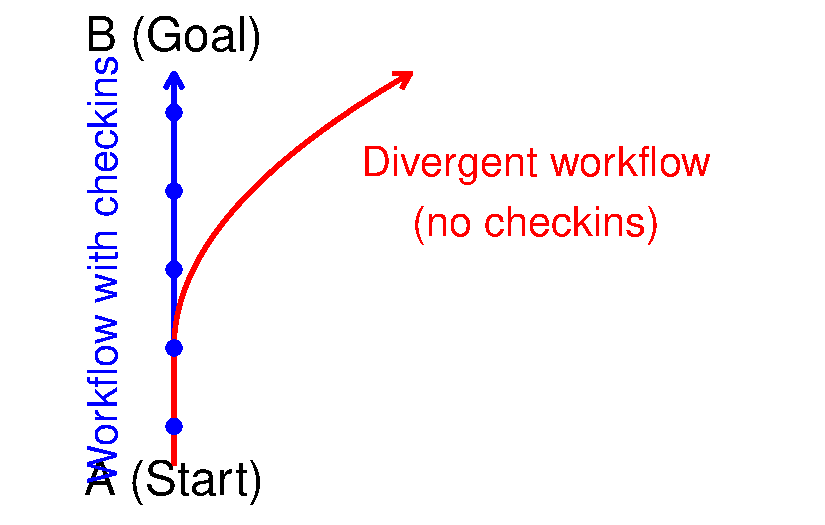
\includegraphics{07-advanced-llm-agents_files/figure-pdf/unnamed-chunk-1-1.pdf}

Have a readme with clear steps that you attach as a prompt is also
helpful for Agent mode. It helps it stay on topic.

Agent mode also allows installation of additional tools, which we'll
explore later.

\bookmarksetup{startatroot}

\chapter{General principles for effective use of LLMs and AI
assistants}\label{general-principles-for-effective-use-of-llms-and-ai-assistants}

\begin{quote}
Take all your problems and rip 'em apart\\
Carry them off in a shopping cart\\
Another thing you should've known from the start\\
The problems in hand are lighter than at heart\ldots{}\\
And another thing you have to know in this world\\
Cut up your hair, straighten your curls\\
Well, your problems hide in your curls
\end{quote}

\emph{Little Acorns by The White Stripes}

If you have a curly problem you need to break it into small parts. And
let's be honest, most real data analysis problems are curly problems.

\textbf{Breaking your problems into small parts} is my number one piece
of advice for any interaction you have with LLMs and AI assistants.

Number two \textbf{is being clear and specific}. Let's look at how these
apply in the context of data analysis

\section{Break your problem down into smaller
parts}\label{break-your-problem-down-into-smaller-parts}

What statistical problems might I run into if I want to build a
statistical model that predicts fish abundance from coral cover?

There's many examples available of how LLMs can reason effectively if
they are encouraged to work through a problem step-by-step, whereas they
guess (some would say hallucinate) the answer if just asked the question
straight up.

Here's a stats motivated example for you to try. Underwater cameras and
deep learning image analysis are used to count fish on surveys, but
\href{TODO\%20add\%20ref}{when fish are in high densities the algorithms
can overcount the number of fish}.

Let's see if the LLM can figure out the logic of adjusting for the
overcounting bias.

Straight-up question:

\begin{tcolorbox}[enhanced jigsaw, coltitle=black, breakable, toptitle=1mm, titlerule=0mm, bottomtitle=1mm, colframe=quarto-callout-note-color-frame, left=2mm, leftrule=.75mm, title=\textcolor{quarto-callout-note-color}{\faInfo}\hspace{0.5em}{Note}, opacityback=0, colback=white, opacitybacktitle=0.6, bottomrule=.15mm, arc=.35mm, rightrule=.15mm, toprule=.15mm, colbacktitle=quarto-callout-note-color!10!white]

I have a regression that finds snapper abundance increases by an average
of 2.5 fish per 10\% increase in seagrass cover, with an intercept of
zero. But the snapper count data were biased upwards at high density,
with a power relationship that has an exponent of 1.1. What is the
expected abundance at a seagrass cover of 55\%?

\end{tcolorbox}

The correct reasoning is: \texttt{2.5*5.5\ =\ 13.75} predicted fish.
Then we adjust for the overcounting bias:
\texttt{13.75\^{}(1/1.1)\ =\ 10.83} which is the true number.

Options for breaking it down into parts

\begin{tcolorbox}[enhanced jigsaw, coltitle=black, breakable, toptitle=1mm, titlerule=0mm, bottomtitle=1mm, colframe=quarto-callout-note-color-frame, left=2mm, leftrule=.75mm, title=\textcolor{quarto-callout-note-color}{\faInfo}\hspace{0.5em}{Note}, opacityback=0, colback=white, opacitybacktitle=0.6, bottomrule=.15mm, arc=.35mm, rightrule=.15mm, toprule=.15mm, colbacktitle=quarto-callout-note-color!10!white]

Think step-by-step to solve this problem: I have a regression that finds
snapper abundance increases by an average of 2.5 fish per 10\% increase
in seagrass cover, with an intercept of zero. But the snapper count data
were biased upwards at high density, with a power relationship that has
an exponent of 1.1. What is the expected abundance at a seagrass cover
of 55\%?

\end{tcolorbox}

\begin{tcolorbox}[enhanced jigsaw, coltitle=black, breakable, toptitle=1mm, titlerule=0mm, bottomtitle=1mm, colframe=quarto-callout-note-color-frame, left=2mm, leftrule=.75mm, title=\textcolor{quarto-callout-note-color}{\faInfo}\hspace{0.5em}{Note}, opacityback=0, colback=white, opacitybacktitle=0.6, bottomrule=.15mm, arc=.35mm, rightrule=.15mm, toprule=.15mm, colbacktitle=quarto-callout-note-color!10!white]

I have a regression that finds snapper abundance increases by an average
of 2.5 fish per 10\% increase in seagrass cover, with an intercept of
zero. But the snapper count data were biased upwards at high density,
with a power relationship that has an exponent of 1.1. What is the
expected abundance at a seagrass cover of 55\%? Use chain-of-thought
reasoning to answer

\end{tcolorbox}

\begin{tcolorbox}[enhanced jigsaw, coltitle=black, breakable, toptitle=1mm, titlerule=0mm, bottomtitle=1mm, colframe=quarto-callout-note-color-frame, left=2mm, leftrule=.75mm, title=\textcolor{quarto-callout-note-color}{\faInfo}\hspace{0.5em}{Note}, opacityback=0, colback=white, opacitybacktitle=0.6, bottomrule=.15mm, arc=.35mm, rightrule=.15mm, toprule=.15mm, colbacktitle=quarto-callout-note-color!10!white]

Think like the White Stripes in their song Little Acorns to solve this
problem: Think step-by-step to solve this problem: I have a regression
that finds snapper abundance increases by an average of 2.5 fish per
10\% increase in seagrass cover, with an intercept of zero. But the
snapper count data were biased upwards at high density, with a power
relationship that has an exponent of 1.1. What is the expected abundance
at a seagrass cover of 55\%?

\end{tcolorbox}

If you have an option for a `thinking' or `reasoning' model available,
try the first prompt again, but use a reasoning model. These use a
different computation process that does more reasoning.

I tested this with Sonnet and GPT 4.1 models in copilot ask mode.
Without the step-by-step instruction they sometimes got it write and
sometimes got it wrong. Often the wrong answers were because they
applied the bias in the wrong direction (ie \texttt{13.75\^{}1.1}). With
a thinking model it got it correct more often.

\section{Be clear, specific and give lots of
details}\label{be-clear-specific-and-give-lots-of-details}

There's a trade-off between spending mental energy on writing a prompt
and writing a prompt that gets you an accurate answer from the LLM. In
general our brains are trying to minimize the amount of writing we do,
so we don't write enough or write clearly enough to get good performance
out of the LLM.

Some commentators have noted that the over-use of the term
`hallucination'. You often find if you ask the same question again, but
with clearer language and more details you'll get an accurate answer. So
is an inaccurate answer really a hallucination (making something up) or
is it just the LLM answering based on insufficient information?

Let's look at a couple of examples.

Clear your script of any plotting code and variable names (if using
VScode) and try getting a GC to create a plot of two variables in our
dataframe. Try this prompt, you can add it as a comment to use inline
code completions, just ask it in `ask mode' (or equivalent) or bring up
the inline chat window (cmd/cntrl-i)

\begin{tcolorbox}[enhanced jigsaw, coltitle=black, breakable, toptitle=1mm, titlerule=0mm, bottomtitle=1mm, colframe=quarto-callout-note-color-frame, left=2mm, leftrule=.75mm, title=\textcolor{quarto-callout-note-color}{\faInfo}\hspace{0.5em}{Note}, opacityback=0, colback=white, opacitybacktitle=0.6, bottomrule=.15mm, arc=.35mm, rightrule=.15mm, toprule=.15mm, colbacktitle=quarto-callout-note-color!10!white]

Plot branching coral cover against distance to logponds.

\end{tcolorbox}

Did the code work without human intervention? Without the context the AI
won't know the variable names. A better prompt would reference the
variable names:

\begin{tcolorbox}[enhanced jigsaw, coltitle=black, breakable, toptitle=1mm, titlerule=0mm, bottomtitle=1mm, colframe=quarto-callout-note-color-frame, left=2mm, leftrule=.75mm, title=\textcolor{quarto-callout-note-color}{\faInfo}\hspace{0.5em}{Note}, opacityback=0, colback=white, opacitybacktitle=0.6, bottomrule=.15mm, arc=.35mm, rightrule=.15mm, toprule=.15mm, colbacktitle=quarto-callout-note-color!10!white]

Plot cb\_cover against dist\_to\_logging\_km

\end{tcolorbox}

or even better

\begin{tcolorbox}[enhanced jigsaw, coltitle=black, breakable, toptitle=1mm, titlerule=0mm, bottomtitle=1mm, colframe=quarto-callout-note-color-frame, left=2mm, leftrule=.75mm, title=\textcolor{quarto-callout-note-color}{\faInfo}\hspace{0.5em}{Note}, opacityback=0, colback=white, opacitybacktitle=0.6, bottomrule=.15mm, arc=.35mm, rightrule=.15mm, toprule=.15mm, colbacktitle=quarto-callout-note-color!10!white]

Make a geom\_point with cb\_cover on the y-axis and
dist\_to\_logging\_km on the x-axis

\end{tcolorbox}

Now let's try a more complex example. If we wan't to get advice on
models for analyzing how the number of fish relates to coral cover we
could ask:

\begin{tcolorbox}[enhanced jigsaw, coltitle=black, breakable, toptitle=1mm, titlerule=0mm, bottomtitle=1mm, colframe=quarto-callout-note-color-frame, left=2mm, leftrule=.75mm, title=\textcolor{quarto-callout-note-color}{\faInfo}\hspace{0.5em}{Note}, opacityback=0, colback=white, opacitybacktitle=0.6, bottomrule=.15mm, arc=.35mm, rightrule=.15mm, toprule=.15mm, colbacktitle=quarto-callout-note-color!10!white]

How could I test the relationship between coral cover and fish?

\end{tcolorbox}

(If trying this in Ask mode make sure you have no data or scripts
attached, which may add the extra context it needs).

Sometimes if you do the above the LLM won't even realize you are asking
for a statistical `test' and may give you an answer for computer
programming tests.

Slight better:

\begin{tcolorbox}[enhanced jigsaw, coltitle=black, breakable, toptitle=1mm, titlerule=0mm, bottomtitle=1mm, colframe=quarto-callout-note-color-frame, left=2mm, leftrule=.75mm, title=\textcolor{quarto-callout-note-color}{\faInfo}\hspace{0.5em}{Note}, opacityback=0, colback=white, opacitybacktitle=0.6, bottomrule=.15mm, arc=.35mm, rightrule=.15mm, toprule=.15mm, colbacktitle=quarto-callout-note-color!10!white]

How could I test if there is a statistically significant relationship
between coral cover and fish?

\end{tcolorbox}

But our data are count data, so the statistically best-practice answer
would be a response that specifically accounts for the fact that fish
are abundance counts.

Even better would be to be specific about the data types:

\begin{tcolorbox}[enhanced jigsaw, coltitle=black, breakable, toptitle=1mm, titlerule=0mm, bottomtitle=1mm, colframe=quarto-callout-note-color-frame, left=2mm, leftrule=.75mm, title=\textcolor{quarto-callout-note-color}{\faInfo}\hspace{0.5em}{Note}, opacityback=0, colback=white, opacitybacktitle=0.6, bottomrule=.15mm, arc=.35mm, rightrule=.15mm, toprule=.15mm, colbacktitle=quarto-callout-note-color!10!white]

How could I test if there is a statistically significant relationship
between coral cover and juvenile fish. Fish abundance is my response
variable. Fish abundance was measured by counting fish on surveys of
standard length at 50 different sites. Coral cover was measured as
percent cover at each site?

\end{tcolorbox}

Try each of these a few times and tally up how often you get a good
recommendation for each prompt style. Make sure you start a new chat
window each time. I would consider a good recommendation one that
appropriately models the count data, e.g.~a poisson or negative binomial
GLM. Coral cover is the predictor variable so we don't need to do any
special transforms on that (sometimes the LLMs will recommend you
transform it also).

Note that if you are using a chat interface, rather than API calls, your
interface may have a `memory' which means each new prompt is not
independent of previous prompts. Check the documents for your software
to be sure and turn off memory if possible. If using VSCode you can open
a new window from the `File' menu and then open the GC chat directly
without opening a project folder (so it has no context).

We could make this prompt even better if we prompt to consider issues
that may arise:

\begin{tcolorbox}[enhanced jigsaw, coltitle=black, breakable, toptitle=1mm, titlerule=0mm, bottomtitle=1mm, colframe=quarto-callout-note-color-frame, left=2mm, leftrule=.75mm, title=\textcolor{quarto-callout-note-color}{\faInfo}\hspace{0.5em}{Note}, opacityback=0, colback=white, opacitybacktitle=0.6, bottomrule=.15mm, arc=.35mm, rightrule=.15mm, toprule=.15mm, colbacktitle=quarto-callout-note-color!10!white]

How could I test if there is a statistically significant relationship
between coral cover and juvenile fish. Fish abundance is my response
variable. Fish abundance was measured by counting fish on surveys of
standard length at 50 different sites. Coral cover was measured as
percent cover at each site? Reason step-by-step and identify any
statistical issues that may arise with this analysis.

\end{tcolorbox}

\section{Put everything up front, rather than engaging in
conversation}\label{put-everything-up-front-rather-than-engaging-in-conversation}

LLMs perform better if you explain to them in detail what you want
straight-up, rather than trying to engage in conversation. Tests show
that answers are less accurate if you present the same question over
multiple turns versus giving all the information up front.

The problem with multi-turn conversation is what's called `context
poisoning'. If the LLM doesn't have all the information it will still
try to answer and it may answer wrongly (what some people inaccurately
call hallucinations). Once that incorrect answer is in the context
window (chat thread) it is hard to get the LLM to forget it. The best
thing to do is start the chat thread over again and write a clearer
prompt to start with.

Try the above example again, but break it into parts and get the LLM to
answer each part before progressing.

\begin{tcolorbox}[enhanced jigsaw, coltitle=black, breakable, toptitle=1mm, titlerule=0mm, bottomtitle=1mm, colframe=quarto-callout-note-color-frame, left=2mm, leftrule=.75mm, title=\textcolor{quarto-callout-note-color}{\faInfo}\hspace{0.5em}{Note}, opacityback=0, colback=white, opacitybacktitle=0.6, bottomrule=.15mm, arc=.35mm, rightrule=.15mm, toprule=.15mm, colbacktitle=quarto-callout-note-color!10!white]

\begin{enumerate}
\def\labelenumi{\arabic{enumi}.}
\tightlist
\item
  How could I test if there is a statistically significant relationship
  between coral cover and juvenile fish.
\item
  Fish abundance is my response variable.
\item
  Fish abundance was measured by counting fish on surveys of standard
  length at 50 different sites.
\item
  Coral cover was measured as percent cover at each site
\end{enumerate}

\end{tcolorbox}

Compare the final answers to the answer you got when you put all of that
in one initial single prompt. Note any instances of context poisoning.

The problem gets worse in bigger projects, because as you fill up more
of the context window small problems can be harder to detect and
eliminate from your context window. For example, an incorrect line of
code in a superseded script make make it into copilot's index may
repeatedly haunt you until you get rid of it and the index is updated.

And that's another reason to use git to manage versions, rather than
keeping multiple versions of the same script hanging around (haunting?)
your project directory.

Its ok to engage the assistant in conversation and use it as a problem
solving partner if you're not sure of how to do something. But you
should be aiming to come up with a plan. Once you have the plan, then
write a really good clear prompt to get the final advice.

\section{Overall advice: Over-explain what you want and say it all up
front}\label{overall-advice-over-explain-what-you-want-and-say-it-all-up-front}

Overall the above steps amount to: Over-explaining what you want and
saying it all up front. This probably means more effort on your behalf
than you were hoping.

You can prompt an agent with a command like `Create an academic paper
about fish and coral using this data', but the answer won't be very good
and will be full of inaccuracies.

If you were to write (optionally with AI assistance) detailed
instructions on your project's aims, the details of the data collection
and the analysis you want to do, you could get a long way towards an
accurate first draft of an academic paper. We'll look at the idea of
expanding prompts into specification sheets later on.

\bookmarksetup{startatroot}

\chapter{AI powered analysis
workflows}\label{ai-powered-analysis-workflows}

Now you are familiar with some of the software options, let's look at
how to use these tools in AI powered analysis workflows and some best
practice prompting guidelines.

For the examples here we'll use the benthic survey data, so make sure
you've set up a project and have that data loaded, as in
Chapter~\ref{sec-githubcopilot-chapter} or below:

\begin{Shaded}
\begin{Highlighting}[]
\FunctionTok{library}\NormalTok{(tidyverse)}
\FunctionTok{library}\NormalTok{(readr)}

\NormalTok{dat }\OtherTok{\textless{}{-}} \FunctionTok{read\_csv}\NormalTok{(}\FunctionTok{url}\NormalTok{(}\StringTok{"https://raw.githubusercontent.com/cbrown5/example{-}ecological{-}data/refs/heads/main/data/benthic{-}reefs{-}and{-}fish/fish{-}coral{-}cover{-}sites.csv"}\NormalTok{))}

\FunctionTok{head}\NormalTok{(dat)}
\FunctionTok{summary}\NormalTok{(dat)}
\end{Highlighting}
\end{Shaded}

\section{Recommended data analysis
workflow}\label{recommended-data-analysis-workflow}

LLM prompting is most effectively designed if you have a good idea of
your goal and the workflow or process that needs to be followed to
achieve that goal.

For data analysis I suggest thinking about four stages:

\begin{enumerate}
\def\labelenumi{\arabic{enumi}.}
\tightlist
\item
  \textbf{Select statistical approach}: Determining appropriate
  statistical methods for research questions
\item
  \textbf{Plan implementation}: Designing the analytical workflow and
  code structure
\item
  \textbf{Write code}: Writing the actual code to implement analyses
\item
  \textbf{Guidance on Interpretation}: Understanding and reporting
  results
\end{enumerate}

LLMs perform differently across these components. They excel at code
generation and implementation planning but are less reliable for
selecting appropriate statistical approaches or interpreting complex
results.

LLMs can be used across all of these steps, but we recommend that each
step is treated separately. This encourages informed decision making and
avoids making decisions on the fly. For instance, it is better to design
the statistical analysis prior to setting an agent up to automate the
implementation of that analysis.

The separation of workflow steps also helps prevent overreliance on LLMs
for statistical decisions.

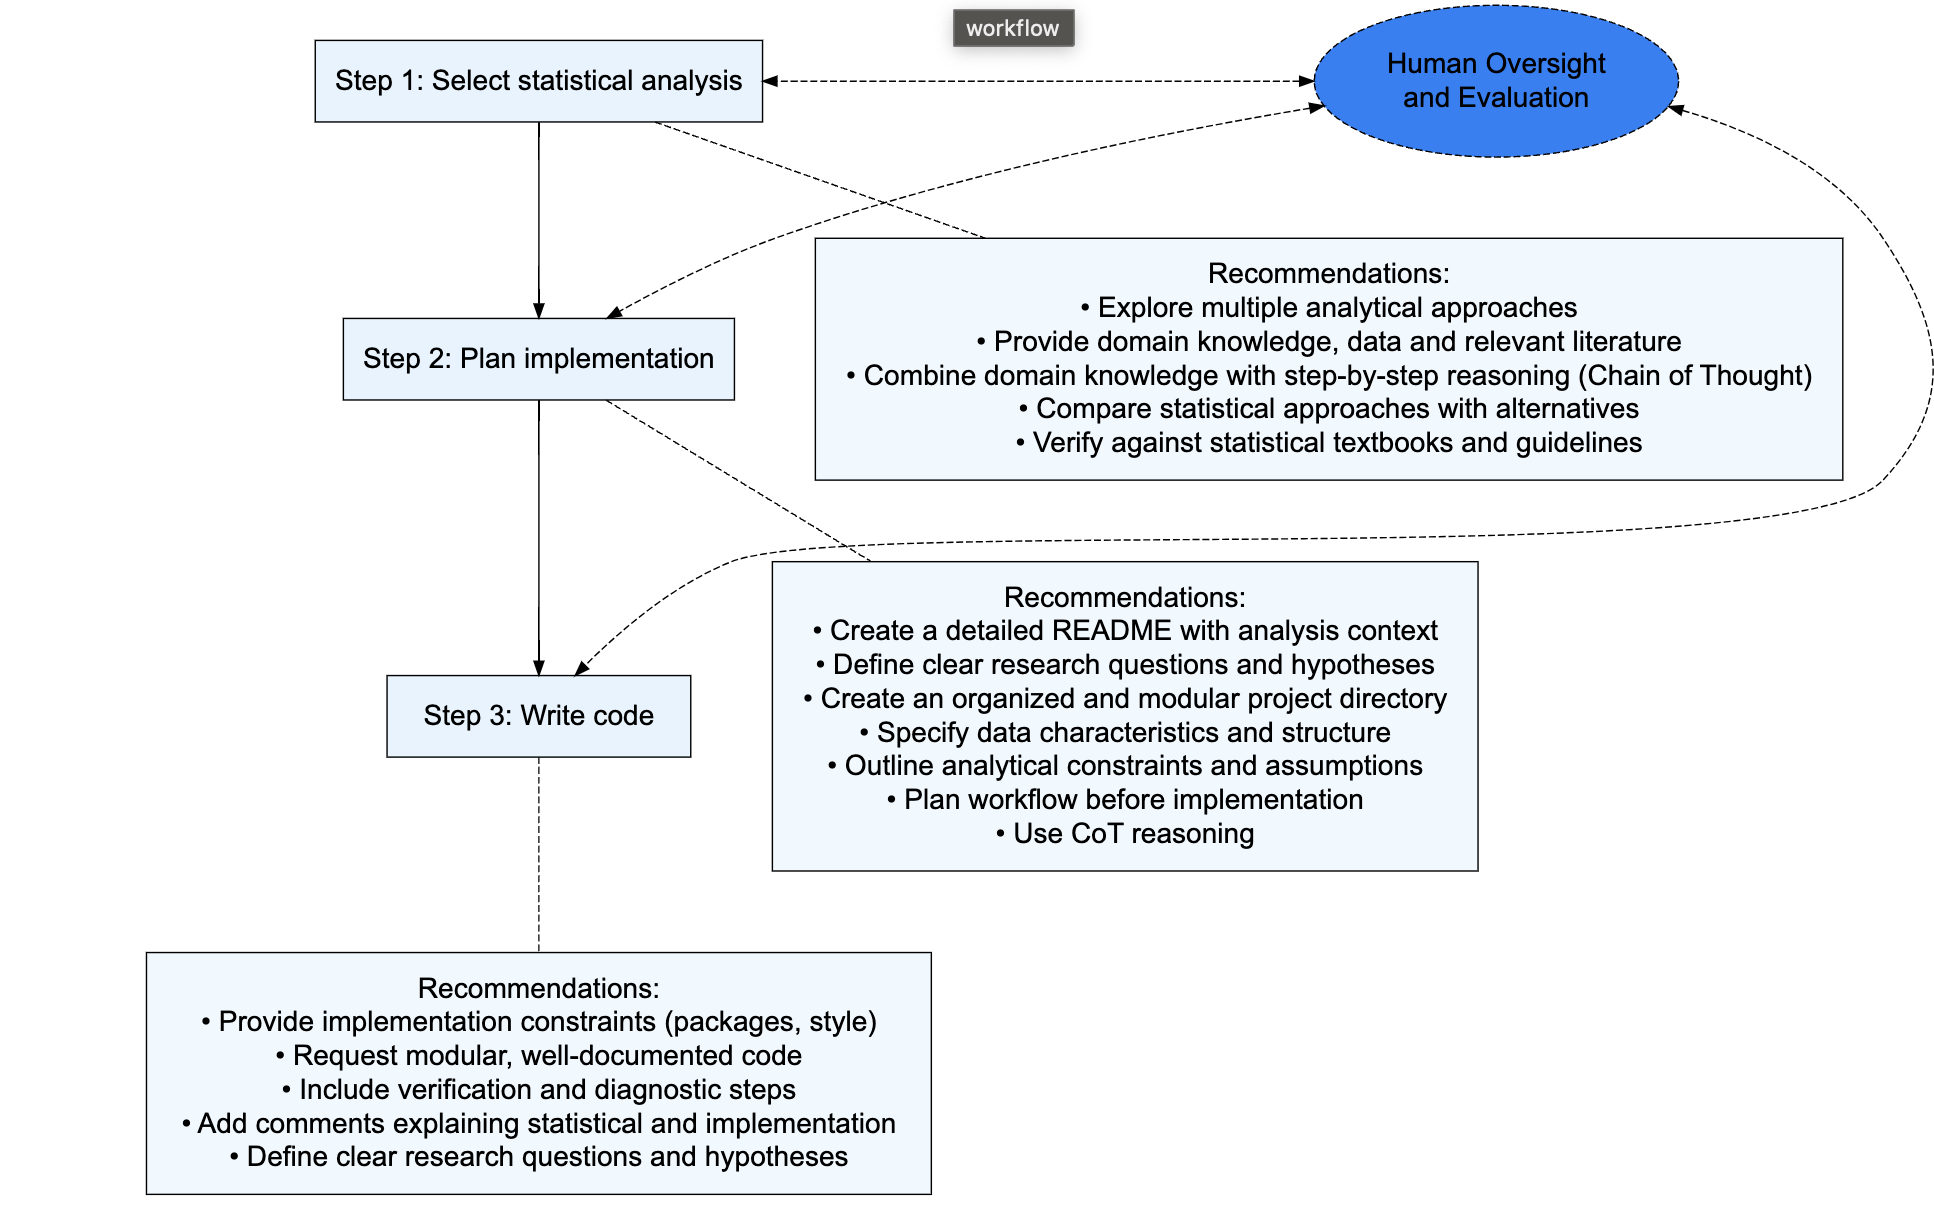
\includegraphics{resources/figure2-brown-spillias.png}

\section{Stages of analysis}\label{stages-of-analysis}

Now let's work through applying that general advice to specific the
stages of analysis I identified.

\section{Selecting a statistical
method}\label{selecting-a-statistical-method}

Its good practice to identify the analysis you want to do, before
thinking about how you write the code for that. Once you have an
approach, follow-up with identifying what packages can implement that
approach.

The limited number of evaluations of LLMs for statistics have found the
biggest improvements for prompts that:

\begin{itemize}
\tightlist
\item
  Include domain knowledge in the prompt
\item
  Include data or summary data in the prompt
\item
  Combine domain knowledge with CoT (but CoT on its own doesn't help)
\end{itemize}

In addition, larger and more up-to-date models tend to be better.
e.g.~try Claude 4.0 or GPT 5.

\textbf{Tip:} LLMs will tend to suggest the most obvious statistical
analyses. If you want to innovate creative new types of analyses you
need to work a bit harder. One way to do this is to mix up your prompts
to try and get cross-disciplinary pollination. For instance, you could
ask it: ``Suggest methods I could use for this analysis, taking
inspiriation from different disciplines such as medicine, psychology and
climate research''.

\subsection{Giving context}\label{giving-context}

As we saw above its a good idea to give the assistant context on your
data, data collection methodology and aims. I recommend writing a
markdown document with all of this information in it. Here's an
\href{link\%20TODO}{example for the analysis of my benthic project}. The
markdown is easy to attach to any request you make to an assistant, or
copy and paste into web forms.

You can of course use the assistant to create the markdown. Try this in
agent mode:

\begin{tcolorbox}[enhanced jigsaw, coltitle=black, breakable, toptitle=1mm, titlerule=0mm, bottomtitle=1mm, colframe=quarto-callout-note-color-frame, left=2mm, leftrule=.75mm, title=\textcolor{quarto-callout-note-color}{\faInfo}\hspace{0.5em}{Note}, opacityback=0, colback=white, opacitybacktitle=0.6, bottomrule=.15mm, arc=.35mm, rightrule=.15mm, toprule=.15mm, colbacktitle=quarto-callout-note-color!10!white]

Write a summary of the meta-data for this database in a new markdown
file {[}attach the csv database{]}

\end{tcolorbox}

Then you can edit the summary to ensure it is accurate.

\subsection{Attaching data or data
summaries}\label{attaching-data-or-data-summaries}

\href{TODO\%20add\%20link}{Attaching the data is proven to improve the
accuracy of statistical recommendations.}

Attaching data works a lot like giving context. The LLM can see what the
data looks like and can often guess variable types from the data field
names or data values.

Large datasets can be hard to attach, because they fill up the context
window. GC agent mode will automatically shorten large data frames if
you attach them.

Or ask the agent to write a script to create a data summary. For
instance try this in agent mode:

\begin{tcolorbox}[enhanced jigsaw, coltitle=black, breakable, toptitle=1mm, titlerule=0mm, bottomtitle=1mm, colframe=quarto-callout-note-color-frame, left=2mm, leftrule=.75mm, title=\textcolor{quarto-callout-note-color}{\faInfo}\hspace{0.5em}{Note}, opacityback=0, colback=white, opacitybacktitle=0.6, bottomrule=.15mm, arc=.35mm, rightrule=.15mm, toprule=.15mm, colbacktitle=quarto-callout-note-color!10!white]

Write a script that creates smaller version of the benthic data that has
only the first six rows of data

\end{tcolorbox}

\textbf{Tip:} If you consult a human statistician they'll usually ask
you lots of questions. LLMs, in contrastwill tend to just give you an
answer, whether or not they have enough context. Say you asked me the
same question you had in your LLM prompt like ``how do see if fish are
related to coral''. There's no way I'd jump in with an answer with so
little information. But the LLM will. So be aware of this shortcoming
and come to prompting pre-prepared with the context it will need to give
you a better answer.

\subsection{Attach domain knowledge}\label{attach-domain-knowledge}

\href{TODO\%20add\%20link}{Domain knowledge is proven to improve the
accuracy of statistical recommendations.}

Domain knowledge on the research question and relevant statistics can
really help refine your approach. If you have a paper that you are
emulating, convert it to markdown so you can attach that as context to
the prompt (e.g.~from a
\href{https://tools.simonwillison.net/jina-reader}{url} or
\href{TODO\%20add\%20link}{pdf}).

Other good sources of domain knowledge are stats tutorial blogs, package
documentation and the R package vignettes. So keep a list of these handy
for when you need them.

Google's LLM notebook is another popular tool for this. Create a
notebook, attach your sources and then ask for a summary. You can then
feed this into your project specific AI assistant as domain knowledge.

\subsection{Web search}\label{web-search}

AI web search tools can help you create customized tutorials for your
stats problem. You can then attach these as context when discussing your
project with the assistant. See the Section~\ref{sec-deepresearch} for
how to use API calls to do this. Many AI web platforms also have web
search features, including chatGPT and copilot. Google is in the process
of adding this option to its search engine.

You'll get the best results if reasoning/thinking modes are enabled. As
these are more energy expensive to run they are often only available for
paid subscriptions. Make sure you read the reasoning information as
well, as its important to understand if the answer is of high quality or
not.

Remember that web search AI doesn't like long prompts, so keep your
prompts short and specific.

Here's a prompt you can try in chatGPT or Copilot (e.g.~in Teams):

\begin{tcolorbox}[enhanced jigsaw, coltitle=black, breakable, toptitle=1mm, titlerule=0mm, bottomtitle=1mm, colframe=quarto-callout-note-color-frame, left=2mm, leftrule=.75mm, title=\textcolor{quarto-callout-note-color}{\faInfo}\hspace{0.5em}{Note}, opacityback=0, colback=white, opacitybacktitle=0.6, bottomrule=.15mm, arc=.35mm, rightrule=.15mm, toprule=.15mm, colbacktitle=quarto-callout-note-color!10!white]

Research the peer-reviewed academic literature to find the most robust
methods for analysing ecological count data.

\end{tcolorbox}

\section{Plan implementation and project
structure}\label{plan-implementation-and-project-structure}

Repeat after me:

\begin{quote}
I will keep my data analysis code neat and organized. I will keep my
data analysis code neat and organized. I will keep my data analysis code
neat and organized.
\end{quote}

If you're like most of us, you probably code as you go and don't spend a
lot of time organizing what you've created. You may end up with a script
that's 1000s of lines long and spans data import, wrangling, initial
visuals, analysis, verification and plotting.

The worst cases I've seen are scripts that don't even evaluate in order,
like students who tell me `run lines 60-70, then go back to line 20 and
it should work\ldots{}'

Have you ever tried to go back into one of your old projects to fix
something and found it a massive mental struggle to work out what you
did? Well that is a problem for the AI assistant too. You're filling its
context window up with irrelevant junk and its going to have a hard time
giving you good advice.

Organized code is good for future you, its good for other scientists
using your code, its good for repeatability AND its good for getting
better help from AI assistants.

Its more work to do, but the good news is that the time cost is more
than made up with the time savings from using the AI. The AI can even
help you be more organized.

So my next step is to plan what you do, before you do it. This means
thinking about the high level steps you'll have to go through to
complete your analysis.

\subsection{Directory structure}\label{directory-structure}

There's no single way to organize your project, the main thing is to be
organized. I keep a folder on my computer with a template. Inside that
folder I have these files and directories:

\begin{verbatim}
glm-test-case/
├──  readme.md           # This readme file with project documentation
├──  .gitignore           # Standard gitignore for R projects
├──  LICENSE
├── data/                    # Data files and intermediate datasets
├── initial-prompt.md       # Initial project prompt and requirements
├── outputs/                # Generated output files
│   └── plots/              # Diagnostic plots and visualization outputs (PNG files)
└── scripts/                # R scripts for data analysis and modeling
\end{verbatim}

You might want to add more nesting if it's a complex project, such as
project with both spatial and non-spatial databases.

\subsection{Readme file for the assistant (and
you)}\label{readme-file-for-the-assistant-and-you}

Here's an example from my readme file, which gives instructions for the
agent for how to structure and navigate the project.

It is helpful to be specific about:

\begin{itemize}
\tightlist
\item
  Folder structure
\item
  Variable names and meta-data
\item
  Code organisation
\item
  Code style
\end{itemize}

Here's an example from one of my readme files that has the above
elements.

\begin{tcolorbox}[enhanced jigsaw, coltitle=black, breakable, toptitle=1mm, titlerule=0mm, bottomtitle=1mm, colframe=quarto-callout-note-color-frame, left=2mm, leftrule=.75mm, title=\textcolor{quarto-callout-note-color}{\faInfo}\hspace{0.5em}{Instructions for the agent}, opacityback=0, colback=white, opacitybacktitle=0.6, bottomrule=.15mm, arc=.35mm, rightrule=.15mm, toprule=.15mm, colbacktitle=quarto-callout-note-color!10!white]

\section{Instructions for the agent}\label{instructions-for-the-agent-1}

The agent will produce a report that answers the above questions. The
report will include a description of the data, the methods used for
analysis, and the results of the analysis. The code will be written as R
scripts.

Each script should be modular and save intermediate results as datafiles
and figures. The final report must be written in Rmarkdown format. The
figures will be imported using markdown syntax,
e.g.~\texttt{!{[}{]}(outputs/plots/figure1.png)}. Don't use R code for
figures in the markdown report. Summary tables should be imported from
.csv files and created using the \texttt{knitr::kable()} function in
Rmarkdown. The report must include the following sections:

\begin{itemize}
\tightlist
\item
  Study aims
\item
  Data methodology
\item
  Analysis methodology
\item
  Results

  \begin{itemize}
  \tightlist
  \item
    Model selection and verification
  \item
    Model fit statistics
  \item
    Plots of predicted fish abundance (log-link scale) based on the
    final model, with confidence intervals
  \item
    Relevant statistics (r2, p-values, etc.)
  \end{itemize}
\end{itemize}

The agent is must produce diagnostic plots and a separate report on the
model diagnostics.

\subsection{Tech context}\label{tech-context}

\begin{itemize}
\tightlist
\item
  We will use the R program
\item
  tidyverse packages for data manipulation
\item
  ggplot2 for data visualization
\item
  use \texttt{theme\_set(theme\_classic())} for plots
\item
  Use the \texttt{MASS} package for the negative binomial model, however
  don't load it globally with \texttt{library(MASS)}, instead use
  \texttt{MASS::glm.nb()} to avoid namespace conflicts.
\item
  Use \texttt{visreg} package for plotting model effects and confidence
  intervals,
  e.g.~\texttt{visreg::visreg(m2,\ "CB\_cover",\ "soft\_cover",\ gg=TRUE,\ scale\ =\ \textquotesingle{}linear\textquotesingle{})}
\end{itemize}

Keep your scripts short and modular to facilitate debugging. Don't
complete all of the steps below in one script. Finish scripts where it
makes sense and save intermediate datasets.

When using Rscript to run R scripts in terminal put quotes around the
file, e.g.~\texttt{Rscript\ "1\_model.R"}

\subsection{Workflow}\label{workflow}

\begin{enumerate}
\def\labelenumi{\arabic{enumi}.}
\tightlist
\item
  Create a todo list and keep track of progress
\item
  Data processing including standardizing coral variables by number of
  points
\item
  Model selection and verification, produce diagnostic plots
\item
  Model diagnostic plots markdown report
\item
  Create plots of predictions from the final model
\item
  Write report in markdown format
\end{enumerate}

\subsection{Directory structure}\label{directory-structure-1}

\begin{verbatim}
glm-test-case/
├── data/                    # Processed data files and intermediate datasets
├── fish-coral.csv          # Raw data file with fish and coral cover measurements
├── glm-readme.md           # This readme file with project documentation
├── initial-prompt.md       # Initial project prompt and requirements
├── outputs/                # Generated output files
│   └── plots/              # Diagnostic plots and visualization outputs (PNG files)
└── scripts/                # R scripts for data analysis and modeling
\end{verbatim}

Put the .rmd reports in the top-level directory.

\end{tcolorbox}

Have a go at writing your own readme file, then using an assistant to
complete the analysis. You will also want to include
\href{https://raw.githubusercontent.com/cbrown5/example-ecological-data/refs/heads/main/readme.md}{meta-data}
and project aims. You can pick your own project aims, but one example
might be a project that aims to test if fish abundance depends on coral
cover.

Once you have your readme, you can attach it (or open it then click new
chat). Given all the context you've provided you can just write
something simple like:

\begin{tcolorbox}[enhanced jigsaw, coltitle=black, breakable, toptitle=1mm, titlerule=0mm, bottomtitle=1mm, colframe=quarto-callout-note-color-frame, left=2mm, leftrule=.75mm, title=\textcolor{quarto-callout-note-color}{\faInfo}\hspace{0.5em}{Note}, opacityback=0, colback=white, opacitybacktitle=0.6, bottomrule=.15mm, arc=.35mm, rightrule=.15mm, toprule=.15mm, colbacktitle=quarto-callout-note-color!10!white]

Help me plan R code to implement this analysis.

\end{tcolorbox}

Or

\begin{tcolorbox}[enhanced jigsaw, coltitle=black, breakable, toptitle=1mm, titlerule=0mm, bottomtitle=1mm, colframe=quarto-callout-note-color-frame, left=2mm, leftrule=.75mm, title=\textcolor{quarto-callout-note-color}{\faInfo}\hspace{0.5em}{Note}, opacityback=0, colback=white, opacitybacktitle=0.6, bottomrule=.15mm, arc=.35mm, rightrule=.15mm, toprule=.15mm, colbacktitle=quarto-callout-note-color!10!white]

Help me plan the workflow and scripts to implement this analysis

\end{tcolorbox}

\section{Writing the code}\label{writing-the-code}

Once you're happy with the plan, you can get copilot to implement it.
There's roughly three ways to do this, with increasing levels of
automation

\begin{enumerate}
\def\labelenumi{\arabic{enumi}.}
\tightlist
\item
  Start creating the code yourself, using inline editing and copilot
  edit to help write bits of the code
\item
  Instruct an AI agent to complete the tasks in the readme, manually
  checking in and editing the code as you go
\item
  Full `vibe-coding' which means you ask an AI agent to complete the
  task and just accept all of its suggestions.
\end{enumerate}

Vibe coding isn't recommended for scientific projects, more on that
later.

\textbf{Tip:} We are using the readme.md is copilot's memory. This means
the assitant always has the context it needs across different chat
sessions (where it would otherwise forget). So its important to keep the
readme updated. Its also useful to help you remember if you come back to
the project some months or years later.

A few more tips for this stage of the analysis.

As you go attach datasets or domain knowledge as neccessary,
particularly if the assistant can't access that information from your
readme.

You can get the assistant to write tests for your datasets. Such as
checking joins worked properly and you didn't duplicate or lose data.

\section{Suggested workflows}\label{suggested-workflows}

\subsection{Suggested workflow for new
analyses}\label{suggested-workflow-for-new-analyses}

Here's a workflow I've found works well if I'm doing an analysis that is
new to means

\begin{enumerate}
\def\labelenumi{\arabic{enumi}.}
\item
  Read the literature to identify the appropriate analysis for the
  research question and data.
\item
  Once I've narrowed down the options I look for useful domain
  knowledge: vignettes, manuals or blogs that have suitable R examples.
\item
  Start a new folder, setting up the directory and readme as descriped
  in this workshop.
\item
  Use copilot to implement the analysis, attaching data summaries and
  the domain knowledge to get the best prompts.
\end{enumerate}

\subsubsection{Suggested workflow for analyses I know
well}\label{suggested-workflow-for-analyses-i-know-well}

Much the same as above, just less planning and you don't need to search
the literature because you know what you want to do. If you save useful
domain knowledge when you see it you will also have the documents on
hand to support the assistant.

\subsection{Iterating}\label{iterating}

Ecological modelling is a creative art with rules. The rules are the
scientific method, the medium is math, logic and code. You can view AI
as part of this creative scientific process, rather than a replacement
for the human.

Use an agent to create multiple complete versions of your project. You
can then compare them to get ideas. You can also continuously refine the
prompt to get what you want as you go.

Add it as a tool inyour belt, not a replacement. Talking to clleagues,
reading, sitting on a board looking at the ocean, having showers
etc\ldots{} are all stil important.

Create same thing multiple times and compare

\bookmarksetup{startatroot}

\chapter{Best practices project
setup}\label{best-practices-project-setup}

This chapter focuses on establishing a project structure and workflow
that can get the most out of your LLM assistants.

\section{Project organization}\label{project-organization}

Its helpful to set-up your projects in an organized and modularised way.
In my experience most R users write most of their analysis in one long
script. Don't do this. It will be hard for `future you' to navigate. If
its hard for a human to navigate, it will also be hard for the
assistant. Here's how I set-up my projects.

\subsection{General guidance}\label{general-guidance}

\begin{itemize}
\tightlist
\item
  Create a new folder for each new project.
\item
  Optional but recommended: Initiliaze a git repo in that folder (I use
  github desktop).
\item
  Set-up folders and files in an organized way
\item
  Ideally put the data in this folder also. However, large datasets or
  sensitive data can be kept in other folders.
\item
  Keep scripts short and modularized (e.g one for data analysis, one for
  modelling).
\end{itemize}

Once you have your folder you can make it an Rstudio project (if using
Rstudio) or just use `open folder' in vscode. If want to link multiple
folders in then use VScode workspaces.

If you are not using git (version control), then I recommend you learn.
LLM code editing tools can cause you to lose older versions. So best to
back them up with proper use of git.

\subsection{Project directory structure
example}\label{project-directory-structure-example}

Here's an example of a project directory structure. You don't have to
use this strucutre. the important thing is to be organized.

\begin{verbatim}
my-project/
├── README.md 
├── .gitignore
├── Scripts/ # R code
│   ├── 01_data-prep.R
│   ├── 02_data-analysis.R
│   └── 03_plots.R
├── Shared/       
│   ├── Outputs/
│   │   ├── Figures/
│   │   ├── data-prep/
│   │   └── model-objects/
│   ├── Data/
│   └── Manuscripts/   
└── Private/
\end{verbatim}

\section{The README.md file}\label{the-readme.md-file}

The README.md is the memory for the project. If you use github it will
also be the landing page for your repo, which is handy.

Remember you are writing this for you and the LLMs. So think of it like
a prompt.

Here's an example of some of the information you might want to include
in your readme.

\begin{verbatim}
# PROJECT TITLE

## Summary

## Aims

## Data methodology

## Analysis methodology

## Tech context
- We will use the R program
- tidyverse packages for data manipulation
- ggplot2 for data visualization

Keep your scripts short and modular to facilitate debugging. Don't complete all of the steps below in one script. Finish scripts where it makes sense and save intermediate datasets. 

## Steps
As you go tick of the steps below. 

[ ] Wrangle data
[ ] Fit regression
[ ] Plot verification
[ ] ... 

## Data 

Include meta-data here and file paths. 

## Directory structure 

my-project/
├── README.md 
├── .gitignore
├── Scripts/ # R code
│   ├── 01_data-prep.R
│   ├── 02_data-analysis.R
│   └── 03_plots.R
├── Shared/       
│   ├── Outputs/
│   │   ├── Figures/
│   │   ├── data-prep/
│   │   └── model-objects/
│   ├── Data/
│   └── Manuscripts/   
└── Private/
\end{verbatim}

\section{Example data}\label{example-data}

For the next few chapters we'll work with some ecological data on
benthic marine habitats and fish.

\subsection{Case-study: Bumphead parrotfish, `Topa' in Solomon
Islands}\label{case-study-bumphead-parrotfish-topa-in-solomon-islands}

Bumphead parrotfish (\emph{Bolbometopon muricatum}) are an enignmatic
tropical fish species. Adults of these species are characterized by a
large bump on their forehead that males use to display and fight during
breeding. Sex determination for this species is unknown, but it is
likely that an individual has the potential to develop into either a
male or female at maturity.

Adults travel in schools and consume algae by biting off chunks of coral
and in the process they literally poo out clean sand. Because of their
large size, schooling habit and late age at maturity they are
susceptible to overfishing, and
\href{https://doi.org/10.1007/s00338-019-01801-z}{many populations are
in decline}.

Their lifecycle is characterized by migration from lagoonal reef as
juveniles (see image below) to reef flat and exposed reef habitats as
adults. Early stage juveniles are carnivorous and feed on zooplankton,
and then transform into herbivores at a young age.

\includegraphics{www.seascapemodels.org/predictive-ecological-models/images/bolbo-lifecycle.png}

Image: Lifecycle of bumphead parrotfish. Image by E. Stump and sourced
from \href{http://dx.doi.org/10.1016/j.biocon.2017.04.024}{Hamilton et
al.~2017}.

Until the mid 2010s the habitat for settling postlarvae and juveniles
was a mystery. However, the pattern of migrating from inshore to
offshore over their known lifecycle suggests that the earliest benthic
lifestages (`recruits') stages may occur on nearshore reef habitats.

Nearshore reef habitats are susceptible to degradation from poor water
quality, raising concerns that this species may also be in decline
because of pollution. But the gap in data from the earliest lifestages
hinders further exploration of this issue.

In this course we'll be analyzing the first survey that revealed the
habitat preferences of early juveniles stages of bumphead parrotfish.
These data were analyzed by
\href{http://dx.doi.org/10.1016/j.biocon.2017.04.024}{Hamilton et
al.~2017} and \href{http://dx.doi.org/10.1111/cobi.13079}{Brown and
Hamilton 2018}.

In the 2010s Rick Hamilton (The Nature Conservancy) lead a series of
surveys in the nearshore reef habitats of Kia province, Solomon Islands.
The aim was to look for the recruitment habitat for juvenile bumphead
parrotfish. These surveys were motivated by concern from local
communities in Kia that topa (the local name for bumpheads) are in
decline.

In the surveys, divers swam standardized transects and searched for
juvenile bumphead in nearshore habitats, often along the edge of
mangroves. All together they surveyed 49 sites across Kia.

These surveys were made all the more challenging by the occurrence of
crocodiles in mangrove habitat in the region. So these data are
incredibly valuable.

Logging in the Kia region has caused
\href{http://dx.doi.org/10.1111/cobi.13079}{water quality issues that
may impact nearshore coral habitats}. During logging, logs are
transported from the land onto barges at `log ponds'. A log pond is an
area of mangroves that is bulldozed to enable transfer of logs to
barges. As you can imagine, logponds are very muddy. This damage creates
significant sediment runoff which can smother and kill coral habitats.

Rick and the team surveyed reefs near logponds and in areas that had no
logging. They only ever found bumphead recruits hiding in branching
coral species.

In this course we will first ask if the occurrence of bumphead recruits
is related to the cover of branching coral species. We will then develop
a statistical model to analyse the relationship between pollution from
logponds and bumphead recruits, and use this model to predict pollution
impacts to bumpheads across the Kia region.

The data and code for the original analyses are
\href{https://github.com/cbrown5/BenthicLatent}{available at my github
site}. In this course we will use simplified versions of the original
data. We're grateful to Rick Hamilton for providing the data for this
course.

\section{Example spec sheet}\label{example-spec-sheet}

\begin{verbatim}
# Analysis of fish dependence on coral habitat

## Introduction
This project will ask how abundance of fish juveniles depends on coral cover. The fish we are interested in is *Bolbometopon muricatum*, the bumphead parrotfish. Also known as 'topa' in the local language of our study region. We will analyze survey data from 49 sites, that includes benthic cover surveys and surveys fish abundance at the same locations. We are studying its juvenile habitat. 

## Aims of the analysis 

1. Does fish abundance depend on branching coral cover? 
2. What is the direction and strength of the relationship between fish abundance and branching coral cover? 
3. Does fish abundance depend on soft coral cover? 
4. What is the direction and strength of the relationship between fish abundance and branching coral cover? 

## Data methodology

The data was collected with the point intersect transect method. Divers swam along transects. There were several transects per site.  Along each transect they dropped points and recorded the type of benthic organism (in categories) on that point. Percentage cover for one organism type can then be calculated as the number of points with that organism divided by the total number of points on that transect. In our data we have percent cover of branching corals and percent cover of soft corals. 
Transects were averaged to give a single value for each site. 
At each site divers also counted the number of juvenile 'topa' along dive transects of the same length. 

## Analysis methodology 

We will use generalized linear models to analyze the relationship between topa and the two coral cover types. 
Topa abundance is probably over-dispersed, so we we will need to use a negative binomial family. We will use R and the MASS package: 
\end{verbatim}

MASS::glm.nb(pres.topa \textasciitilde{} CB\_cover*soft\_cover, data =
fish\_coral\_cover\_sites)

\begin{verbatim}

To obtain a final model we should model selection, starting with a full model then working towards simpler models. We will use likelihood ratio tests to compare models. For example the first test would be: 
\end{verbatim}

m1 \textless- MASS::glm.nb(pres.topa \textasciitilde{}
CB\_cover*soft\_cover, data = fish\_coral\_cover\_sites) m2 \textless-
MASS::glm.nb(pres.topa \textasciitilde{} CB\_cover + soft\_cover, data =
fish\_coral\_cover\_sites) anova(m1, m2, test = ``Chisq'')

\begin{verbatim}

Then proceed with m2 if the interaction term is not significant. Elsewise to the next proceed with m1.

On completion of the model selection, we will do model diagnostics. This will include checking residuals and the dispersion parameter. Save these as png files. 

Write a diagnosticis report in an Rmarkdown file. 


## Instructions for the agent

The agent will produce a report that answers the above questions. The report will include a description of the data, the methods used for analysis, and the results of the analysis. The code will be written as R scripts. 

Each script should be modular and save intermediate results as datafiles and figures. The final report must be written in Rmarkdown format. The figures will be imported using markdown syntax, e.g. `![](outputs/plots/figure1.png)`. Don't use R code for figures in the markdown report. 
Summary tables should be imported from .csv files and created using the `knitr::kable()` function in Rmarkdown. 
The report must include the following sections:

- Study aims
- Data methodology
- Analysis methodology
- Results
  - Model selection and verification
  - Model fit statistics
  - Plots of predicted fish abundance (log-link scale) based on the final model, with confidence intervals
  - Relevant statistics (r2, p-values, etc.)

The agent is must produce diagnostic plots and a separate report on the model diagnostics. 

### Tech context
- We will use the R program
- tidyverse packages for data manipulation
- ggplot2 for data visualization
- use `theme_set(theme_classic())` for plots
- Use the `MASS` package for the negative binomial model, however don't load it globally with `library(MASS)`, instead use `MASS::glm.nb()` to avoid namespace conflicts.
- Use `visreg` package for plotting model effects and confidence intervals, e.g. `visreg::visreg(m2, "CB_cover", "soft_cover", gg=TRUE, scale = 'linear')`

Keep your scripts short and modular to facilitate debugging. Don't complete all of the steps below in one script. Finish scripts where it makes sense and save intermediate datasets. 

When using Rscript to run R scripts in terminal put quotes around the file, e.g. `Rscript "1_model.R"`

### Workflow 

1. Create a todo list and keep track of progress
2. Data processing including standardizing coral variables by number of points
3. Model selection and verification, produce diagnostic plots
4. Model diagnostic plots markdown report 
5. Create plots of predictions from the final model
6. Write report in markdown format

### Directory structure 

/```
glm-test-case/
├── data/                    # Processed data files and intermediate datasets
├── fish-coral.csv          # Raw data file with fish and coral cover measurements
├── glm-readme.md           # This readme file with project documentation
├── initial-prompt.md       # Initial project prompt and requirements
├── outputs/                # Generated output files
│   └── plots/              # Diagnostic plots and visualization outputs (PNG files)
└── scripts/                # R scripts for data analysis and modeling
/```

Put the .rmd reports in the top-level directory. 

## Meta data 

### fish-coral.csv

Location: `data/fish-coral.csv`

Variables
- site: Unique site IDs, use to join to benthic_cover.csv
- reef.ID: Unique reef ID
- pres.topa: number of Topa counted (local name for Bolbometopon)
- pres.habili: number of Habili counted (local name for Cheilinus) 
- secchi: Horizontal secchi depth (m), higher values mean the water is less turbid
- flow: Factor indicating if tidal flow was "Strong" or "Mild" at the site
- logged: Factor indicating if the site was in a region with logging "Logged" or without logging "Not logged"
- coordx: X coordinate in UTM zone 57S
- coordy: Y coordinate in UTM zone 57S
- CB_cover: Number of PIT points for branching coral cover
- soft_cover: Number of PIT points for soft coral cover
- n_pts: Number of PIT points at this site (for normalizing cover to get per cent cover)
- dist_to_logging_km: Linear distance to nearest log pond (site where logging occurs) in kilometres. 
\end{verbatim}

\bookmarksetup{startatroot}

\chapter{Writing documents with Quarto and AI
assistants}\label{writing-documents-with-quarto-and-ai-assistants}

Below is my suggested workflow for using quarto to write scientific
papers with the help of AI assistants. I'm currently switching to doing
as many projects as possible with quarto rather than word for a few
reasons:

\begin{enumerate}
\def\labelenumi{\arabic{enumi}.}
\item
  Easier to manage document style
\item
  Easier to manage references
\item
  Workflows that auto-update figures/tables when R code is re-run
\item
  Generative AI integration that is customizable.
\end{enumerate}

Point 3 is great, no more cut and pasting figures into word documents!

Point 4 is the big one. I'm developing my own `writing mentor' scripts
for large language models. Using quarto lets me implement writing advice
specific to science direclty into my manuscripts.

Quarto is `What You See is What you Make', meaning that you write
special syntax for formatting. Once you are used to it, this is way
easier way to manage styles than word.

Another option is Rmarkdown, which is very similar to quarto, just with
fewer features.

The downside is getting your (non-coding) collaborators to edit files in
quarto. This is the biggest bottleneck to my use of quarto/markdown.
Currently I send them word documents then have to manually integrate the
feedback. Or I work in quarto until the near final stages, accepting
comments only, then get them to edit the final manuscript.

For instance,
\href{https://conbio.onlinelibrary.wiley.com/doi/full/10.1111/cobi.13079?casa_token=zF8vihnFfcMAAAAA\%3A9WlbXPCghdwS2WvyRqGjRqYPrng7q4_xPwZvu9K52p6gd_8lWs2qcgrehfg4ehAThC7ni32Ybr02iA}{I
wrote most of this paper in markdown} but had to go to word editing
towards the end so I could get edits from my collaborator (this was all
before AI assistants). Once you've progressed it in word, its hard to go
back to markdown.

Instructions below are high level. There are quite a few pieces of
software you need to do this, so I've linked to tutorials for each
below.

\subsection{1. Download and install an
IDE}\label{download-and-install-an-ide}

Download and install VScode as per Section~\ref{sec-vscodesetup}.

I'm using VScode because of its AI assistant integration. But you could
also use positron if you have issues with VScode or want to use a Posit
product rather than a Microsoft product.

\subsection{2. Get git and github}\label{get-git-and-github}

Install git on your computer. Optionally, get a github account and
connect to that. Git does version control. Github lets you share that
online. If your collaborators are github users then you can also share
edits on documents this way.

Git is also essential if you are using AI assistants. Sometimes they
majorly stuff up your documents, such as over-writing content you want
to keep. So keeping back-ups with git is essential.

\subsection{3. VScode extensions}\label{vscode-extensions}

Install these VScode extentions (or equivalents if you are using
positron, note that many vscode extensions are also compatable with
Positron)

\begin{itemize}
\tightlist
\item
  Quarto extension.
\end{itemize}

Open VSCode and click the four boxes `extension' icon on the LHS then
search and install the Quarto extension.

\subsection{4. Steps for AI integration}\label{steps-for-ai-integration}

Quarto in VScode is great on its own. But if you want to use AI
assistants there's a few more steps.

If you are using quarto or markdown its possible to get large-language
models to help with many paper writing tasks (including the writing).
This is a specialized area though and I've only given basic technical
instructions here. Actually getting it to work well is another topic
altogether and something I'm still developing\ldots{}

Get an API key with an LLM provider see Section~\ref{sec-apikeys}.

Get an AI assistant extension for your IDE. Here I'll assume you are
using the Roo Code extension for VSCode Section~\ref{sec-otheroptions}.

The reason I like Roocode for this is the ability to to create custom
modes, so you can create a mode specific to scientific writing.

\href{https://docs.roocode.com/}{Read the documents/watch the tutorials
and learn how to use Roo Code}

You can now \href{https://docs.roocode.com/features/custom-modes}{create
a custom mode}, e.g.~a `scientific writing mode' in Roo code. As of
writing this requires clicking the mode selection button at the bottom
of the Roo Code Pane, then click the Cog, then the \texttt{+} button to
make a new mode. Then you need to write a `Role Definition' and `Custom
instructions'. For tools I just use `Read Files', `Edit Files' and
unclick the others (will save you money and tokens).

This is the hard part that needs a lot of thought:

In the custom instructions you should write detailed instructions on how
to help an author with scientific writing. For instance, you might want
to put some very strong instructions about not making up references. You
might also put instructions about your particular writing style
preferences. I'm working on a template, but am not yet ready to share
it.

See \href{https://docs.roocode.com/features/custom-modes}{Roo code
documentation} for more advice on custom modes.

You can also create custom modes in VSCode. Open the chat window and
click the cog to access the menu for creating custom modes.

\subsection{5. Using quarto}\label{using-quarto}

Take a tutorial and
\href{https://quarto.org/docs/get-started/hello/rstudio.html}{learn how
to use Quarto}.

For academic paper writing the key things to understand from the Quarto
tutorial are:

\begin{itemize}
\tightlist
\item
  How to knit as word or pdf (pdf requires extra software installations)
\item
  Formatting, headings, bold etc\ldots{}
\item
  YAML frontmatter for styles, linking a bibliography and bibliography
  style
\item
  How to insert images and/or code.
\end{itemize}

\textbf{Note on AI integration} once you are using quarto and Roo Code
you can simply ask Roo Code to do things in your document (like outline
a paper template) by referencing the file (e.g. (\textbf{myfile.qmd?}))
in the prompt box.

Whether this works well for you is another questions. Prompting well
requires a lot of thought and practice. Its not simply going to write a
paper for you. You have to give the AI assistant detailed, specific,
instructions and lots of context.

Note in VSCode as of writing you need to set your quarto window to
`source' mode. The AI assistants generally won't work if its set to
`visual' mode. I recommend memorising the short-cut key to easily flick
between these two modes (cmd-shft-F4 on my computer).

\subsection{6. YAML front matter}\label{yaml-front-matter}

The \texttt{YAML} controls how your qmd document is rendered. Here's an
example of mine:

\begin{verbatim}
---
title: "The paper's title"
format: docx
editor: visual
bibliography: mybib.bib
csl: myjournal.csl
execute: 
  echo: false
  message: false
  warning: false
---
\end{verbatim}

This goes at the top of your document. A few key points.

\texttt{format} controls document type to render this as, here a word
doc.

\texttt{editor} controls how it is viewed in vscode. Options are
\texttt{editor:\ visual} and \texttt{editor:\ source}. Visual looks more
like a word doc, source looks more like markdown. You'll have to save
and re-open the document for this to change.

\texttt{bibliography} links to a bibtex file where your references are
stored.

\texttt{csl} links to a style guide for the bibliography.

More on styles and references below.

\texttt{execute} is controlling how R code is run and if the R code
appears in the document.

\subsection{7. Rendering as a document}\label{rendering-as-a-document}

Use the short-cut key `cmd-shift-K'/`cntrl-shft-k' (mac/windows) to
preview your document. It will also create a rendered version in your
current directory.

Its helpful to set: \texttt{format:\ html} when you are writing the
document, then you get a live preview in vscode. Use
\texttt{format:\ docx} when you want a word document.

Its worth also learning the short-cut `cmd-shft-p'/`cntrl-shft-p', this
brings up searchable actions for all extensions in vscode. The one you
want is `Quarto: preview' which does the same as the shortcut above.

I tend to have minimal R code in my quarto manuscript. Or none at all
(just reference .png files for figures). This keeps rendering quick.
Also your document can get unweildy if there is a lot of text mixed in
with R code.

\subsection{8. Word counts}\label{word-counts}

There are various word count extensions for vscode qmd and md documents.

\subsection{9. Document styles}\label{document-styles}

Getting a word document to follow a particular style is a bit fiddly.
You need to set-up a template word document with styles the include that
as a reference in your YAML.

\href{https://quarto.org/docs/output-formats/ms-word-templates.html}{See
instructions here.}

\subsection{10. Reference manager
integration}\label{reference-manager-integration}

Quarto integrates with many different reference managers.
\href{https://quarto.org/docs/authoring/citations.html}{There's a good
guide here}.

In brief you create a \texttt{.bib} file that has your references in it.
This is then linked in the YAML. The manual way to manage this is just
to create a \texttt{.bib} file and paste bibtext entries directly into
it (available on most journal's pages as a citation format, as well as
google scholar).

e.g.~the bibtext for R looks like this:

\begin{verbatim}
@Manual{Rlanguage,
    title = {R: A Language and Environment for Statistical Computing},
    author = {{R Core Team}},
    organization = {R Foundation for Statistical Computing},
    address = {Vienna, Austria},
    year = {2024},
    url = {https://www.R-project.org/},
  }
\end{verbatim}

Then in quarto you just type \texttt{@} and a dropdown of all your
references will appear. \texttt{@Manual\{Rlanguage,} the Rlanguage bit
is the CiteKey that will appear in the dropdown. So \texttt{@Rlanguage}
will insert that reference into the bibliography and the citation at
that place in the document.

You can streamline the process of gathering and managing references with
a reference manager.

My workflow in Zotero is as follows:

\begin{itemize}
\tightlist
\item
  Open Zotero on my computer
\item
  Go to journal webpage for paper
\item
  Use zotero plugin to my browser to grab the citation and save it to a
  library
\item
  Go to my quarto document in VScode
\item
  type \texttt{@} and a drop down of all references in all libraries on
  zotero appears. Pick the one I want.
\item
  Click the \texttt{OK} button which saves that reference into my local
  \texttt{.bib} file.
\end{itemize}

For some reason (that does not seem to be documented in any quarto
tutorials anywhere!) it will find any reference I have anywhere in
zotero and then save that bibtex entry to my local \texttt{.bib} file,
so it is now accessible for use in my quarto doc. This only works if I
have zotero open and use \texttt{editor:\ visual} in the YAML.

There are many other options however.

\subsection{11. Optional AI integration for reference
management}\label{optional-ai-integration-for-reference-management}

You can get AI assistants to help with referencing if you keep your
notes on papers linked to your references. For instance, you could keep
your notes on references in the bibtex field for \texttt{notes}.
Alternatively you could create another quarto/markdown document that has
a header for each citation tag along with its notes in a structured way:

\begin{verbatim}
## Rlanguage 

### What it is

The R software for scientific computing. 

### Usage

Citation for the R software. Use this at least once in every paper where i've used R for statistics

## edgar2023continent

### What is it

Key paper that shows Australia is losing its marine biodiversity. 

### Usage

Cite this as evidence that Australia is losing coastal marine biodiversity and as evidence that climate change is causing marine biodiversity loss
\end{verbatim}

It doesn't matter how you do this, so long as you follow a consistent
structure. I've used the CiteKey as the main header for each reference
entry. Then I've put in markdown sections about each paper and why I
might wnat to cite it. Then you can get Roo Code to help with inserting
references.

Note that if you are using the \texttt{.bib} directly just be careful
not to plagiarise! Roo Code might insert excerpts from the
abstracts/titles directly into your written document, which is a no-no
for publishing.

\bookmarksetup{startatroot}

\chapter{Cost and security}\label{cost-and-security}

This chapter addresses important practical considerations when using
LLMs for R programming:

\section{Cost considerations}\label{cost-considerations}

\begin{itemize}
\tightlist
\item
  PIs need to consider cost and impact on research budget
\item
  e.g.~Copilot subscription free for students
\item
  Tools like Roo Code can be more expensive (pay per use as using API).
\item
  Still less than a person (currently)
\item
  e.g.~processing 6000 abstracts to extract data for a lit review might
  cost about USD300 (including cost of developing prompts)
\item
  Strategies for optimizing token usage
\item
  Balancing cost with capability requirements
\end{itemize}

AI companies are running at a loss and its quite likely that costs will
go up in future. The aim right now is to get us all dependent on the
technology, so that we have to keep paying in future (another reason I
think its improtant our own countries develop these capaibilites, and
that we also need to strive to be capable to work in AI free ways as
well. )

\section{API security}\label{api-security}

\begin{itemize}
\tightlist
\item
  Managing API keys and credentials
\item
  Sanitizing inputs to remove sensitive information
\item
  Local vs.~cloud-based LLM solutions
\item
  Auditing and monitoring LLM interactions
\end{itemize}

\section{Agent security}\label{agent-security}

\begin{itemize}
\tightlist
\item
  Can run code on your computer
\item
  Be careful what it is doing
\item
  Read prompts before running them
\end{itemize}

Computer enginners, thinking probabilistically

\section{Lethal trifecta for prompt injection
attacks}\label{lethal-trifecta-for-prompt-injection-attacks}

The \href{https://simonwillison.net/2025/Aug/9/bay-area-ai/}{Lethal
Trifecta for prompt injection attacks} (coined by Simon Williamson) is
access to private data, ability to communicate externally and exposure
to untrusted content.

What can happen is that if your agent can read untrusted sources, those
sources may contain malicious prompts. These prompts could convince the
agent to do things like send or post your personal data to the hacker or
create malicious code that runs on your computer.

You want to be sure your agents can't do these three things at once.
Remember sensitive data includes your name, username, phone number,
email, API keys as well as sensitive research data.

\bookmarksetup{startatroot}

\chapter{Ethics and copyright}\label{ethics-and-copyright}

There's several fundamental ethical issues we should discuss related to
the development of LLMs and AI in general.

\begin{itemize}
\tightlist
\item
  That LLMs use considerable energy and water resources
\item
  That many LLMs have probably been trained on copyright data, so there
  is IP theft
\item
  That concentration of LLM capabilities in a few big companies may
  contribute to rising inequality
\item
  That LLMs have inherent biases and will change the way science is
  done, possibly for the worse.
\end{itemize}

I've developed a
\href{https://docs.google.com/forms/d/e/1FAIpQLSeK7KInwDKSgCEKYSj5xFVeT4gGIxr4cCDCRqYl29i6n_-eOA/viewform}{little
quiz to help you think about your personal ethics.}

\section{Who's responsible for
mistakes?}\label{whos-responsible-for-mistakes}

You are.

When to vibe code, when not to vibe code.

\section{Impacts on learning}\label{impacts-on-learning}

Does AI make our brains lazy?
\href{https://www.nature.com/articles/d41586-025-02005-y}{One study
found} less engagement and deep thinking for students who had access to
chatGPT for writing an essay compared to students who just had web
searches or had no internet connectivity.

I think the upshot is using it deliberatley and being careful not to
replace your own creativity.

\section{Sustainability}\label{sustainability}

Training LLMs costs millions of dollars, much of this cost is energy
use. Further, the data centres for training and running LLMs need water
for cooling. Asking a finished LLM questions uses much less energy, but
cumulatively across the globe it adds up to a lot. Here are a few
informative statistics I found online:

From
\href{https://www.forbes.com/sites/cindygordon/2024/03/12/chatgpt-and-generative-ai-innovations-are-creating-sustainability-havoc/}{Forbes}:

\begin{itemize}
\tightlist
\item
  ``ChatGPT's daily power usage is nearly equal to 180,000 U.S.
  households, each using about twenty-nine kilowatts.''
\item
  Microsoft emissions have risen 30\% since 2020 due to data centers
\item
  AI prompts use 10x more energy than a traditional google search
\end{itemize}

To put it in context I did some calculations on my personal usage. I
estimate the prompting I do through copilot each year will cost about
\textbf{2.32 kg of C02} and about \textbf{1000 litres of water}. (this
is lower bound, as I also using LLMs for other tasks).

To put that in context, flying the 1.5 hours from Halifax to Montreal is
about 172kg of emissions, driving 15 minutes is about 3 kg. So I'm using
approximately 10 less than a short flight, or the same as driving to
work once. 1000L is equivalent to taking about 22 5-minute showers.

Of course, the carbon cost is global, whereas the water cost is
localised (Probably to US data centres, so by using this resource I'm
really just making the water problem worse for Americans. )

So its not a huge increase in my personal energy use. But cumulatively
across the globe it is a lot.

More generally,
\href{https://www.pnas.org/doi/abs/10.1073/pnas.1508353112}{humanities
energy use is growing exponential}. Despite renewables and so on,
ultimately our planet won't be able to sustain this energy drawdown.
LLMs are part of that trend of growing energy use. At some point we need
to start using less energy, or the biosphere will become depleted and
return to a
\href{https://www.pnas.org/doi/abs/10.1073/pnas.1508353112}{`moon like
rock' in one study's words}.

Here's my personal belief.

If we're smart humanity will use this technology to find ways to make
our use of the planet more sustainable and ultimately save water and
energy. Just like we should have been using fossil fuels to develop a
transition to lasting sustainanle energy use. So you can guess how
likely that is to happen\ldots{}

Its the reason I'm teaching this course. I don't personally think that
LLMs make our lives better, or humanity more sustainable. They just
raise the bar on the rate of progress.

You can bet industries are using this technology to improve their
productivity (= greater environmental impacts). I believe as
environmental scientists we need to try to keep up. Ultimately we need
progress on local to planetary sustainability (environmental scientists)
to outpace the development of the industries that are environmentally
unsustainable.

\section{Model biases}\label{model-biases}

This is a big one. I recommend everyone read this perspective on the
\href{https://www.nature.com/articles/s41586-024-07146-0}{`Illusion of
Understanding'}

Its important that we don't become too reliant on AI for our work.
That's why I'm teaching and promoting thoughtful use.

Some key points:

\begin{itemize}
\tightlist
\item
  We need to maintain and grow research fields that aren't convenient to
  do with AI, not just grow the stuff that's easy with AI
\item
  We need to push ourselves as individuals to not `be lazy' and rely on
  AI too much. There is still great value in human learning. This
  requires mental energy, for instance, you will know something better
  if you write it yourself rather than write it with AI.
\item
  We need to be aware of biases in the content AI generates
\end{itemize}

For statistics these biases are likely to be a preference for well-known
methods developed by Western science. So you should still read the
literature broadly and avoid using AI, or prompt it in different ways,
if you truly want to create novel statitistics (as opposed to using it
to do statistics on a study that is otherwise novel data etc\ldots)

\section{Rising inequality}\label{rising-inequality}

AI development is currently concentrated in the USA and profits for LLM
use go to American companies. (USA is itself a country with massive
inequality issues!). So the extent to LLMs replaces labour will redirect
income and taxes from jobs in countries to American companies.

It is likely that the current low cost of LLM use will not continue.
Companies are running at a loss in order to gain market share. So be
careful how dependent you become on the LLMs and what that budget is
replacing in your research budgets.

I personally beleive that our own countries should be developing our own
LLM products and resources. Even if they are not `industry leading' they
can still be highly effective for specific tasks. There are open-source
models available that can fill this role.

\section{Copyright}\label{copyright}

Many LLMs have been trained on pirated books. The
\href{https://www.forbes.com/sites/danpontefract/2025/03/25/authors-challenge-metas-use-of-their-books-for-training-ai/}{extent
to which this is recognized by law is still in court}.

For me personally its frustrating that I spent years developing a
statistics blog (which was open-access, but I appreciated attribution),
but now that information has been mined by LLMs. Thus AI companies are
profiting from our collective knowledge.

It is an even worse situation for authors who's livelihoods and careers
depend on their copyrighted works.

Copilot does in theory block itself from writing code that might be
copyrighted. However, the efficacy of this system is unclear (it seems
to just be a command in the system prompt). So be careful. Here are some
recommendations for individuals

\begin{itemize}
\tightlist
\item
  In general you own works you create with an LLM.
\item
  This also means you have the liability for any works you create (not
  normally an issue in environmental sciences).
\item
  e.g.~you couldn't blame the LLM if you had to retract a paper due to
  incorrect statistics.
\item
  You should acknolwedge LLM use in academic publications, and what you
  used it for.
\item
  Always look for original sources references, e.g.~don't `cite' the LLM
  for use of a GLM, use a textbook or reputable source (Zuur's books are
  good for this!)
\end{itemize}

\section{Managing data privacy}\label{managing-data-privacy}

Any prompt you send to an LLM provider is going to the server of an AI
company (e.g.~Google). So its important to be mindful of what
information you are including in your prompts.

The data you send (including text data) will be covered by the privacy
policy of the LLM provider. Some services claim to keep your data
private (e.g.~the Copilot subscription my University has). Public
services will tend to retain the right to use any data you enter as
prompts.

This means if you put your best research ideas into chatGPT, its
possible that it will repeat them later to another user who asks similar
questions. So be mindful of what you are writing.

Before using an LLM to help with data analysis, be sure you understand
the IP and ethical considerations involved with that data. For instance,
if you have human survey data you may not be allowed to send that to a
foreign server, or reveal any information to an LLM.

In that case you have three options.

\subsubsection{Option 1: Locally hosted
LLM}\label{option-1-locally-hosted-llm}

Use a locally hosted LLM. We won't cover setting these up in this
workshop. Locally hosted LLMs run on your computer. They can be suitable
for simpler tasks and if you have a reasonably powerful GPU. Downsides
are they do not have the performance of the industry leading LLMs and
response times can be slower.

\subsubsection{Option 2: Keep data seperate from code
development.}\label{option-2-keep-data-seperate-from-code-development.}

Use the LLM to help generate code to analyse the data, but do not give
the LLM the data or the results. I would recommend keeping the data in a
different directory altogether (ie not your project directory), so that
LLM agents don't inadvertently access the raw data. You also want to be
sure that the LLM isn't returning results of data analysis to itself
(and therefore you reveal private information to the LLM).

It can be helpful to generate some simulated data to use for code
development, so there is no risk of violating privacy.

\subsubsection{Option 3: Ignore sensitive
folders}\label{option-3-ignore-sensitive-folders}

Some LLM agents can be directed to ignore specific folders. e.g.~You
could add a command to ignore a folder to
\href{https://docs.github.com/en/copilot/customizing-copilot/adding-repository-custom-instructions-for-github-copilot}{copilot
custom instructions}, Roo Code has a \texttt{.rooignore} file for this.

However, remember prompts are not 100\% precise (unlike real code), so
there's still the chance the LLM will go in those folders. So be
careful, if its really sensitive keep it elsewhere on your computer, and
always check its actions before you approve them.

\subsubsection{Option 4: Service with no data retention
policy}\label{option-4-service-with-no-data-retention-policy}

Openrouter has a `no data retention' option you can click in the
profile, it will filter providers to those with NDR rules.

\section{Supplement: Calculations of personal environmental impact from
using
LLMs}\label{supplement-calculations-of-personal-environmental-impact-from-using-llms}

A ChatGPT request uses 2.9 watt-hour. So say that's similar cost for
coding applicatoins (probably more due to the additional context we are
loading with every prompt). Then looking at my chat history I had 14
conversations in the last week (not counting in-line editing). Average
was 3x requests per conversation, so in a year that equals: 2.9 * 14 * 3
* 52 = 6.33 kW-hours In USA energy cost on Average is 367 grams C02 per
kW-hour. (https://www.eia.gov/tools/faqs/faq.php?id=74\&t=11) So my
conservative estimated yearly usage for coding: 6.33 x 367 = 2.32 kg C02
For comparison flying the 1.5 hours from Halifax to Montreal is about
172kg of emissions. So my personal annual emissions for coding are
perhaps about 10x than a short plane flight. Water is used for cooling
in data centres: ``A single ChatGPT conversation uses about fifty
centilitres of water, equivalent to one plastic bottle.'' Based on
calculations above, this equates to about 1000L per year. That's
equivalent to about 22 x 5-minute showers.

\bookmarksetup{startatroot}

\chapter{Code for fish and benthic
analysis}\label{code-for-fish-and-benthic-analysis}

\section{Read in the data from an online
source}\label{read-in-the-data-from-an-online-source}

\begin{Shaded}
\begin{Highlighting}[]
\FunctionTok{library}\NormalTok{(readr)}

\CommentTok{\# URLs for datasets}
\NormalTok{benthic\_cover\_url }\OtherTok{\textless{}{-}} \StringTok{"https://raw.githubusercontent.com/cbrown5/example{-}ecological{-}data/refs/heads/main/data/benthic{-}reefs{-}and{-}fish/benthic\_cover.csv"}
\NormalTok{benthic\_variables\_url }\OtherTok{\textless{}{-}} \StringTok{"https://raw.githubusercontent.com/cbrown5/example{-}ecological{-}data/refs/heads/main/data/benthic{-}reefs{-}and{-}fish/benthic\_variables.csv"}
\NormalTok{fish\_coral\_cover\_sites\_url }\OtherTok{\textless{}{-}} \StringTok{"https://raw.githubusercontent.com/cbrown5/example{-}ecological{-}data/refs/heads/main/data/benthic{-}reefs{-}and{-}fish/fish{-}coral{-}cover{-}sites.csv"}

\CommentTok{\# Local file paths}
\NormalTok{benthic\_cover\_path }\OtherTok{\textless{}{-}} \StringTok{"data/benthic\_cover.csv"}
\NormalTok{benthic\_variables\_path }\OtherTok{\textless{}{-}} \StringTok{"data/benthic\_variables.csv"}
\NormalTok{fish\_coral\_cover\_sites\_path }\OtherTok{\textless{}{-}} \StringTok{"data/fish{-}coral{-}cover{-}sites.csv"}

\CommentTok{\# Download and save datasets}
\NormalTok{benthic\_cover }\OtherTok{\textless{}{-}} \FunctionTok{read\_csv}\NormalTok{(benthic\_cover\_url)}
\FunctionTok{write\_csv}\NormalTok{(benthic\_cover, benthic\_cover\_path)}

\NormalTok{benthic\_variables }\OtherTok{\textless{}{-}} \FunctionTok{read\_csv}\NormalTok{(benthic\_variables\_url)}
\FunctionTok{write\_csv}\NormalTok{(benthic\_variables, benthic\_variables\_path)}

\NormalTok{fish\_coral\_cover\_sites }\OtherTok{\textless{}{-}} \FunctionTok{read\_csv}\NormalTok{(fish\_coral\_cover\_sites\_url)}
\FunctionTok{write\_csv}\NormalTok{(fish\_coral\_cover\_sites, fish\_coral\_cover\_sites\_path)}
\end{Highlighting}
\end{Shaded}

\section{Convert the benthic data to a wide format data
frame}\label{convert-the-benthic-data-to-a-wide-format-data-frame}

\begin{Shaded}
\begin{Highlighting}[]
\CommentTok{\# Load required libraries}
\FunctionTok{library}\NormalTok{(tidyverse)}

\CommentTok{\# Load benthic cover data}
\NormalTok{benthic }\OtherTok{\textless{}{-}} \FunctionTok{read\_csv}\NormalTok{(}\StringTok{"data/benthic\_cover.csv"}\NormalTok{)}

\CommentTok{\# Calculate proportional cover per transect}
\NormalTok{benthic }\OtherTok{\textless{}{-}}\NormalTok{ benthic }\SpecialCharTok{\%\textgreater{}\%}
    \FunctionTok{mutate}\NormalTok{(}\AttributeTok{prop\_cover =}\NormalTok{ cover }\SpecialCharTok{/}\NormalTok{ n.pts)}

\CommentTok{\# Average proportional cover by site and habitat type}
\NormalTok{benthic\_site }\OtherTok{\textless{}{-}}\NormalTok{ benthic }\SpecialCharTok{\%\textgreater{}\%}
    \FunctionTok{group\_by}\NormalTok{(site, code) }\SpecialCharTok{\%\textgreater{}\%}
    \FunctionTok{summarise}\NormalTok{(}\AttributeTok{mean\_prop\_cover =} \FunctionTok{mean}\NormalTok{(prop\_cover, }\AttributeTok{na.rm =} \ConstantTok{TRUE}\NormalTok{), }\AttributeTok{.groups =} \StringTok{"drop"}\NormalTok{)}

\CommentTok{\# Pivot to wide format: one row per site, columns for each habitat type}
\NormalTok{benthic\_wide }\OtherTok{\textless{}{-}}\NormalTok{ benthic\_site }\SpecialCharTok{\%\textgreater{}\%}
    \FunctionTok{pivot\_wider}\NormalTok{(}\AttributeTok{names\_from =}\NormalTok{ code, }\AttributeTok{values\_from =}\NormalTok{ mean\_prop\_cover)}

\CommentTok{\# View result}
\FunctionTok{print}\NormalTok{(}\FunctionTok{head}\NormalTok{(benthic\_wide))}
\NormalTok{readr}\SpecialCharTok{::}\FunctionTok{write\_csv}\NormalTok{(benthic\_wide, }\AttributeTok{file =} \StringTok{"data/benthic\_wide.csv"}\NormalTok{)}
\end{Highlighting}
\end{Shaded}

\section{Join the benthic and fish
datasets}\label{join-the-benthic-and-fish-datasets}

\begin{Shaded}
\begin{Highlighting}[]
\FunctionTok{library}\NormalTok{(tidyverse)}
\FunctionTok{library}\NormalTok{(readr)}
\NormalTok{fish }\OtherTok{\textless{}{-}} \FunctionTok{read\_csv}\NormalTok{(}\StringTok{"data/fish{-}coral{-}cover{-}sites.csv"}\NormalTok{)}
\NormalTok{benthic\_wide }\OtherTok{\textless{}{-}} \FunctionTok{read\_csv}\NormalTok{(}\StringTok{"data/benthic\_wide.csv"}\NormalTok{)}

\NormalTok{dat }\OtherTok{\textless{}{-}} \FunctionTok{left\_join}\NormalTok{(fish, benthic\_wide, }\AttributeTok{by =} \StringTok{"site"}\NormalTok{)}
\end{Highlighting}
\end{Shaded}





\end{document}
